\chapter{Evaluation}
Im anschließenden Kapitel wird die Güte des VAE basierten Data Augmentation Ansatzes auf den in Kapitel \ref{cpt:datasets} beschriebenen Datensätzen evaluiert. Außerdem wird eine umfassende Analyse des Latent-Spaces vorgeführt. Alle Zufallskomponenten wurden mit Seeds verwendet, um zwischen den Methoden vergleichbare Resultate zu erzielen. Dabei wurden alle Experimente stets für 3 verschiedene Seeds durchgeführt. Anschließend wurden die Ergebnisse der Metriken gemittelt. Alle Hyperparameter wurden innerhalb der Experimente identisch gewählt und für die Gewichtung $\beta$ des KL-Terms wurde keine $\beta$-Normalisation angewandt, wenn nicht anders vermerkt. Trainiert wurde auf einer GeForce RTX 2070 SUPER mit 8 GB VRAM.\\

\section{Metriken}
\begin{table}[hbt]
\centering
\begin{tabular}{l|l|l|l}
\multicolumn{2}{l}{\multirow{2}{*}{}}                                                  & \multicolumn{2}{|c}{ground truth} \\ \cline{3-4}
\multicolumn{2}{l|}{}                                                                   & True                              & False \\ \hline
\rule{0pt}{25pt}\multirow{2}{*}{\rotatebox[origin=c]{90}{predicted}} & \rotatebox[origin=c]{90}{True}  & true-positive (tp) & false-positive (fp) \rule{0pt}{25pt} \\ \cline{2-4} 
\rule{0pt}{25pt} & \rotatebox[origin=c]{90}{False}   & false-negative (fn) & true-negative (tn) \rule{0pt}{25pt}
\end{tabular}
\caption{Üblicherweise beschreibt man in der Klassifikation die Beziehung zwischen Vorhersage eines Modells (\textit{predicted}) und der tatsächlichen Klasse (\textit{ground truth}) über eine Konfusionsmatrix. Basierend darauf ergeben sich mehrere Bewertungs Metriken.}
\end{table}

In der binären Klassifikation dient meist die \textit{Accuracy} Metric als Bewertungsgrundlage. Diese teilt die Anzahl richtig-positiv ($tp$) vorhergesagter Klassen durch die Gesamtanzahl an Beispielen. In der Multi-Class Klassifikation bringt die \textit{Accuracy} jedoch den Nachteil mit, dass sie falsch-positive ($fp$) und falsch-negative ($fn$) nicht berücksichtig. Daher betrachten wird in dieser Arbeit der F-Score als Vergleichsmetrik betrachtet. Der F-Score stellt das harmonische Mittel von "Recall" und "Precision" dar (siehe Gl. \ref{eq:f1_score}).
\begin{align}\label{eq:f1_score}
  precision &= \frac{tp}{tp + fp} \notag\\
  recall &= \frac{tp}{tp + fn} \notag\\
  \textit{f-score} &= 2 \cdot \frac{precision \cdot recall}{precision + recall} \\
         &= \frac{tp}{tp + \frac{1}{2}(fp + fn)} \notag
\end{align}

Im Fall von mehr als zwei Klassen werden verschiedene Durchschnittsmethoden benutzt, um die klassenweisen F-Scores zusammenzurechnen (siehe Gleichung \ref{eq:f_score_averaging}). Da auch imbalancierte Datensätze Teil der Experimente sind, wird der \textit{weighted-F-Score} als Vergleichsmetrik genutzt. Dieser gewichtet die klassenweisen F-Scores nach der Anzahl an Beispielen pro Klasse. $k$ bezeichnet die Anzahl an Klassen und $n_c$ die Anzahl an Beispielen in Klasse $c$. $n$ gibt die Gesamtanzahl Beispiele an.
\begin{align} \label{eq:f_score_averaging}
  \textit{micro-f-score}    &= \frac{\sum_{c=1}^{n} tp_c}{\sum_{c=1}^{n} tp + fp} = \textit{Accuracy} \notag\\
  \textit{macro-f-score}    &= \frac{\sum_{c=1}^{n} f_c}{n} \notag\\
  \textit{weighted-f-score} &= 2 \frac{\sum_{c=1}^{n} f_c \cdot n_c}{n}
\end{align}


\subsection{Few-Shot Szenario}
Für die Evaluation in Few-Shot Szenarien wird die Größe der Trainings-Partition jedes Datensatzes reduziert. Gewählt werden dabei jeweils $n$ Beispiele pro Klasse, mit \\
$n \in \lbrace 2, 3, 4, 5, 10, 20, 30, 50, 100, 200, 500, 1000, 2000\rbrace$. Für 1-Shot Learning ist der Multi-VAE basierte Ansatz nicht praktikabel, da aus einem Beispiel keine Generalisierung über den Datensatz erzielt werden kann. In diesem Fall erzeugt der VAE keine ungesehen Beispiele. Da ebenfalls die Interpolations- und Extrapolations Methoden auf einer nächsten-Nachbar Suche basieren, welche bei nur einem Beispiel nicht möglich ist, werden nur Few-Shot Szenarien ab $n=2$ untersucht.



\section{Latent-Space Analyse}\label{sec:latent_space_analysis}
Für die Analyse des Latent-Space wird aus Gründen der Visualisierung im Folgenden eine Latent-Space Dimension von $d = 2$ betrachtet. Analysiert wird zunächst die Test-Partition des MNIST Datensatzes. Abb. \ref{fig:mnist_latent_space} stellt eine Visualisierung des erlernten Latent-Spaces dar. Zu sehen ist, dass die Encoder Verteilung nahe einer Normalsverteilung $\cN(0, 1)$ liegt. Gleichzeitig ist eine Trennung der verschiedenen Klassen in einzelne Cluster sichtbar. Es fällt auf, dass die beiden Ziffern 4 und 9 weniger deutlich als z.B. 0 und 1 getrennt werden. Offenbar ähneln sich die Merkmale einer 4 und einer 9 also mehr. Dies ist auch in den Rekonstruktionen in Abb. \ref{fig:mnist_recon_4} erkennbar. Auffallend ist, dass einige Klassen einen größeren Teil des Latent-Spaces einnehmen, obwohl die Anzahl der Beispiele pro Klasse im Training identisch war.

\begin{figure}[hbt]
\begin{subfigure}{.5\textwidth}
  \centering
  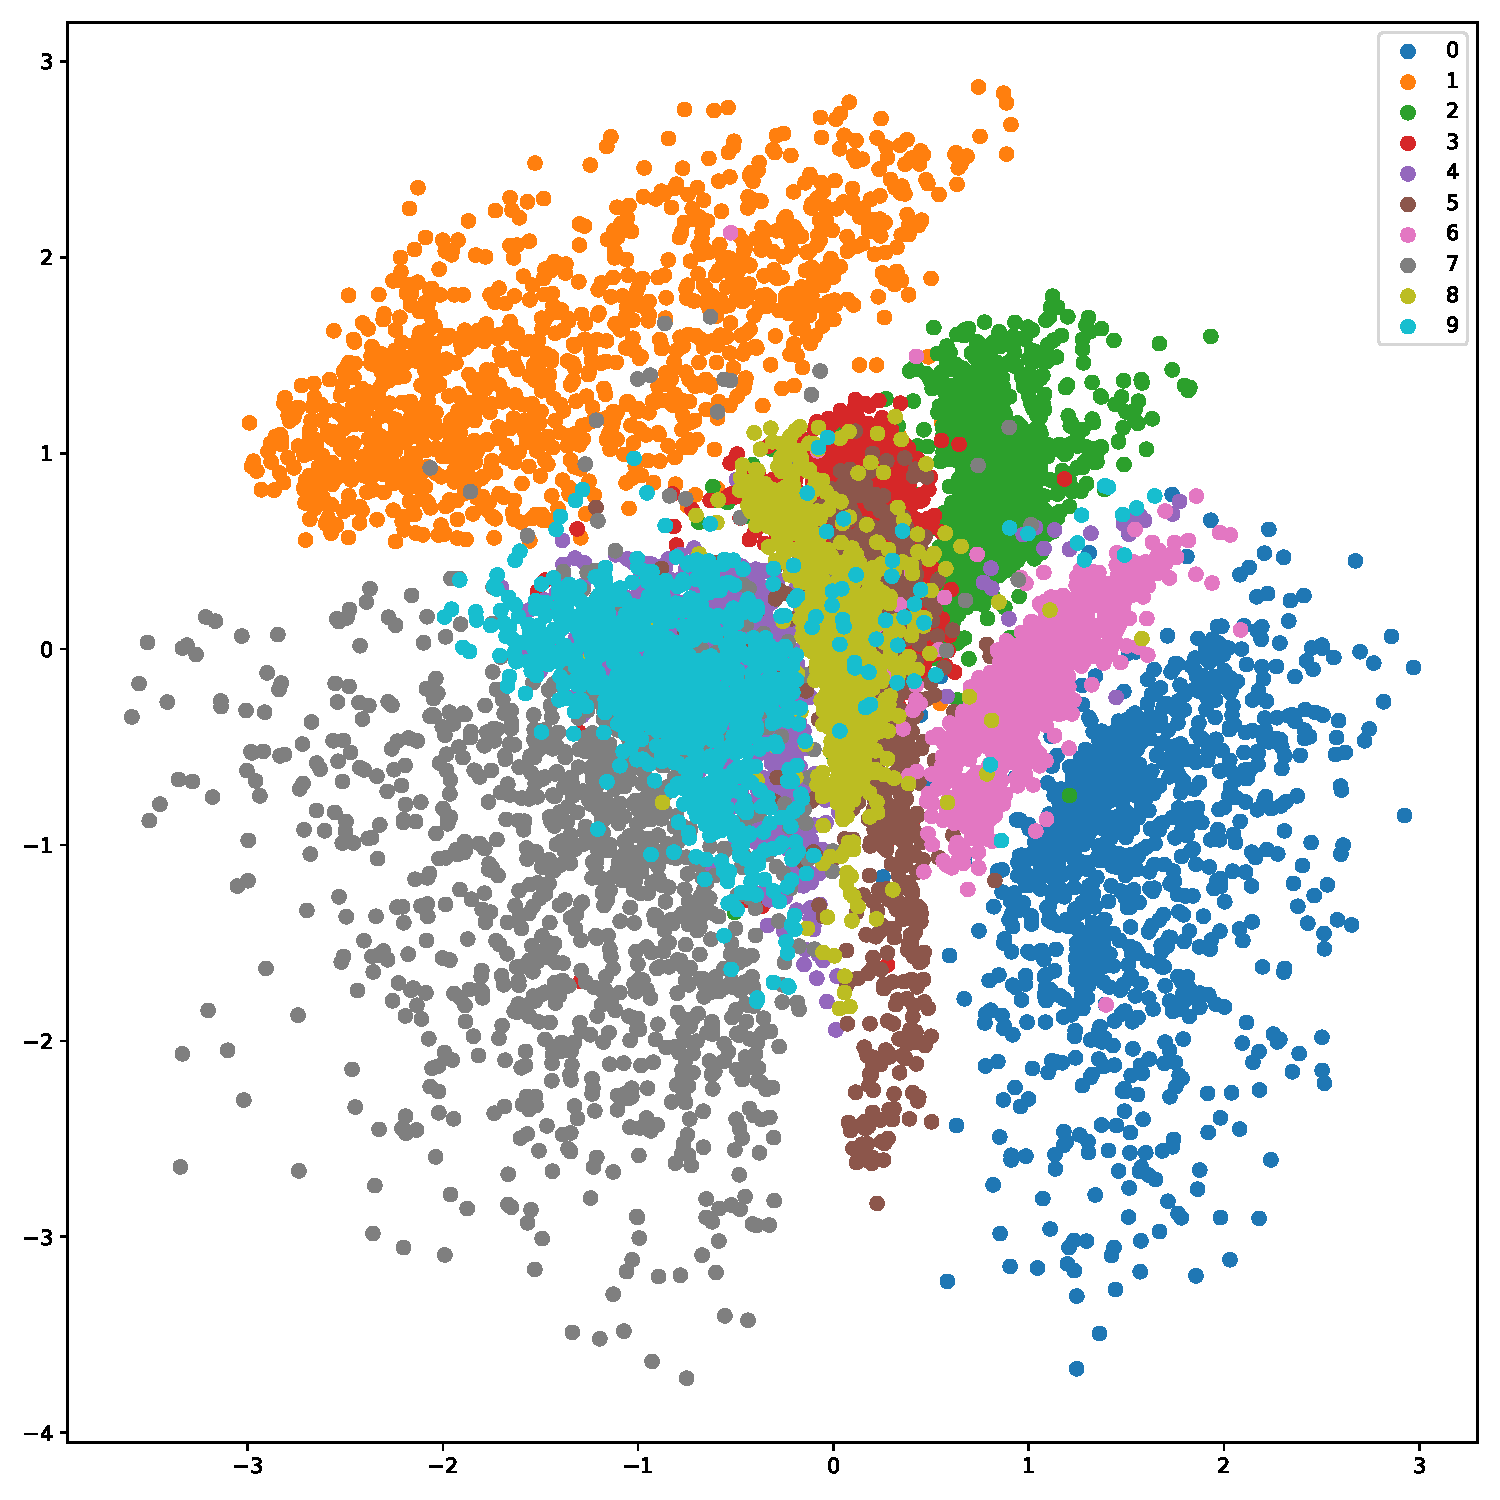
\includegraphics[width=\textwidth]{gfx/evaluation/feature_space/distributions_mnist}
  \caption{Latent Space}
  \label{fig:mnist_latent_space}
\end{subfigure}%
\begin{subfigure}{.5\textwidth}
  \centering
  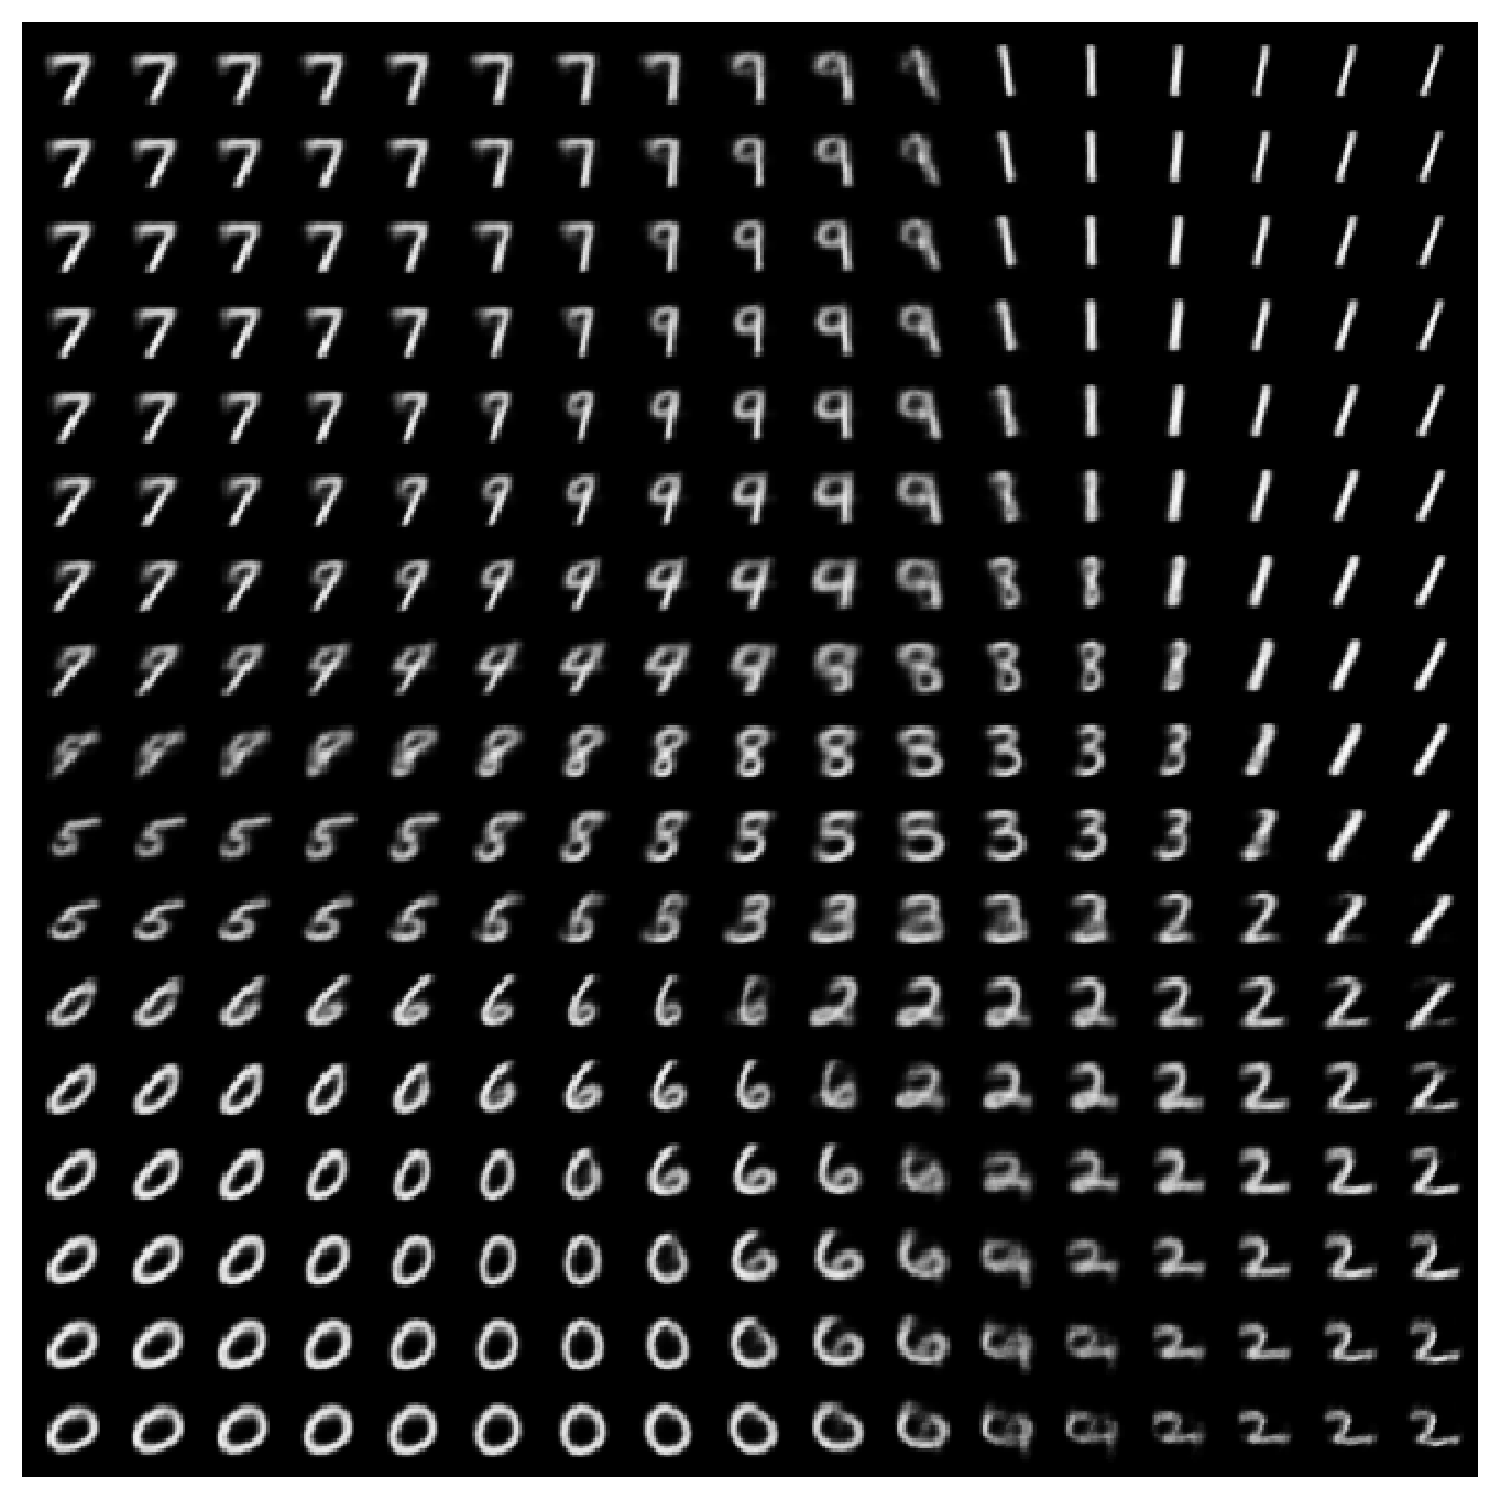
\includegraphics[width=\textwidth]{gfx/evaluation/feature_space/mnist_grid.pdf}
  \caption{Generierte Beispiele}
  \label{fig:mnist_reconstructions}
\end{subfigure}
\caption{(links) Der Latent Space eines Single-VAE auf dem Datensatz MNIST. Trainiert wurde mit $\beta = 0.5$. Zu sehen ist die klare Trennung der Klassen im äußeren Bereich. Nahe 0 sind die Klassen weniger deutlich getrennt. (rechts) Die Rekonstruktionen von Latent-Vektoren aus dem Intervall $(-3, 3)$. Auch hier sind die Rekonstruktionen im äußeren Bereich deutlich schärfer.}
\end{figure}

Abb. \ref{fig:mnist_reconstructions} zeigt die Rekonstruktionen von 2D Latent-Vektoren aus dem Intervall $(-3, 3)$ in beiden Dimensionen. Es ist dieselbe Trennung wie schon im Latent-Space sichtbar. An den Grenzen zwischen zwei Clustern sind außerdem Mischformen von Klassen zu sehen.

\begin{figure}[hbt]
  \centering
  
\includegraphics[width=\textwidth]{gfx/evaluation/feature_space/mnist_4}
  \caption{Rekonstruktionen verschiedener Original Ziffern 4 beim Single-VAE. Trainiert wurde mit $\beta = 0.5$. Zu sehen ist das Problem bei Überlappungen von Klassen im Latent-Space. Die Rekonstruktionen sind nicht eindeutig einer 4 oder 9 zuordbar, da durch die geringe Latent-Space Dimension ein zu hoher Informationsverlust mit einhergeht. Höheren Latent-Space Dimensionen verringern diesen Effekt.}
  \label{fig:mnist_recon_4}
\end{figure}

In Abb. \ref{fig:extrapolation_feature_space} ist die Funktionsweise des Interpolations- bzw. Extrapolations-Samplings gezeigt. Eine Erkenntnis ist, dass bei diesen Sampling Methoden immer garantiert ist, aus der Nähe von Originalbeispielen zu sampeln. Damit ergeben sich mehr plausible Rekonstruktionen. \\
\begin{figure}[hbt]
\centering
\begin{subfigure}{.5\textwidth}
  \centering
  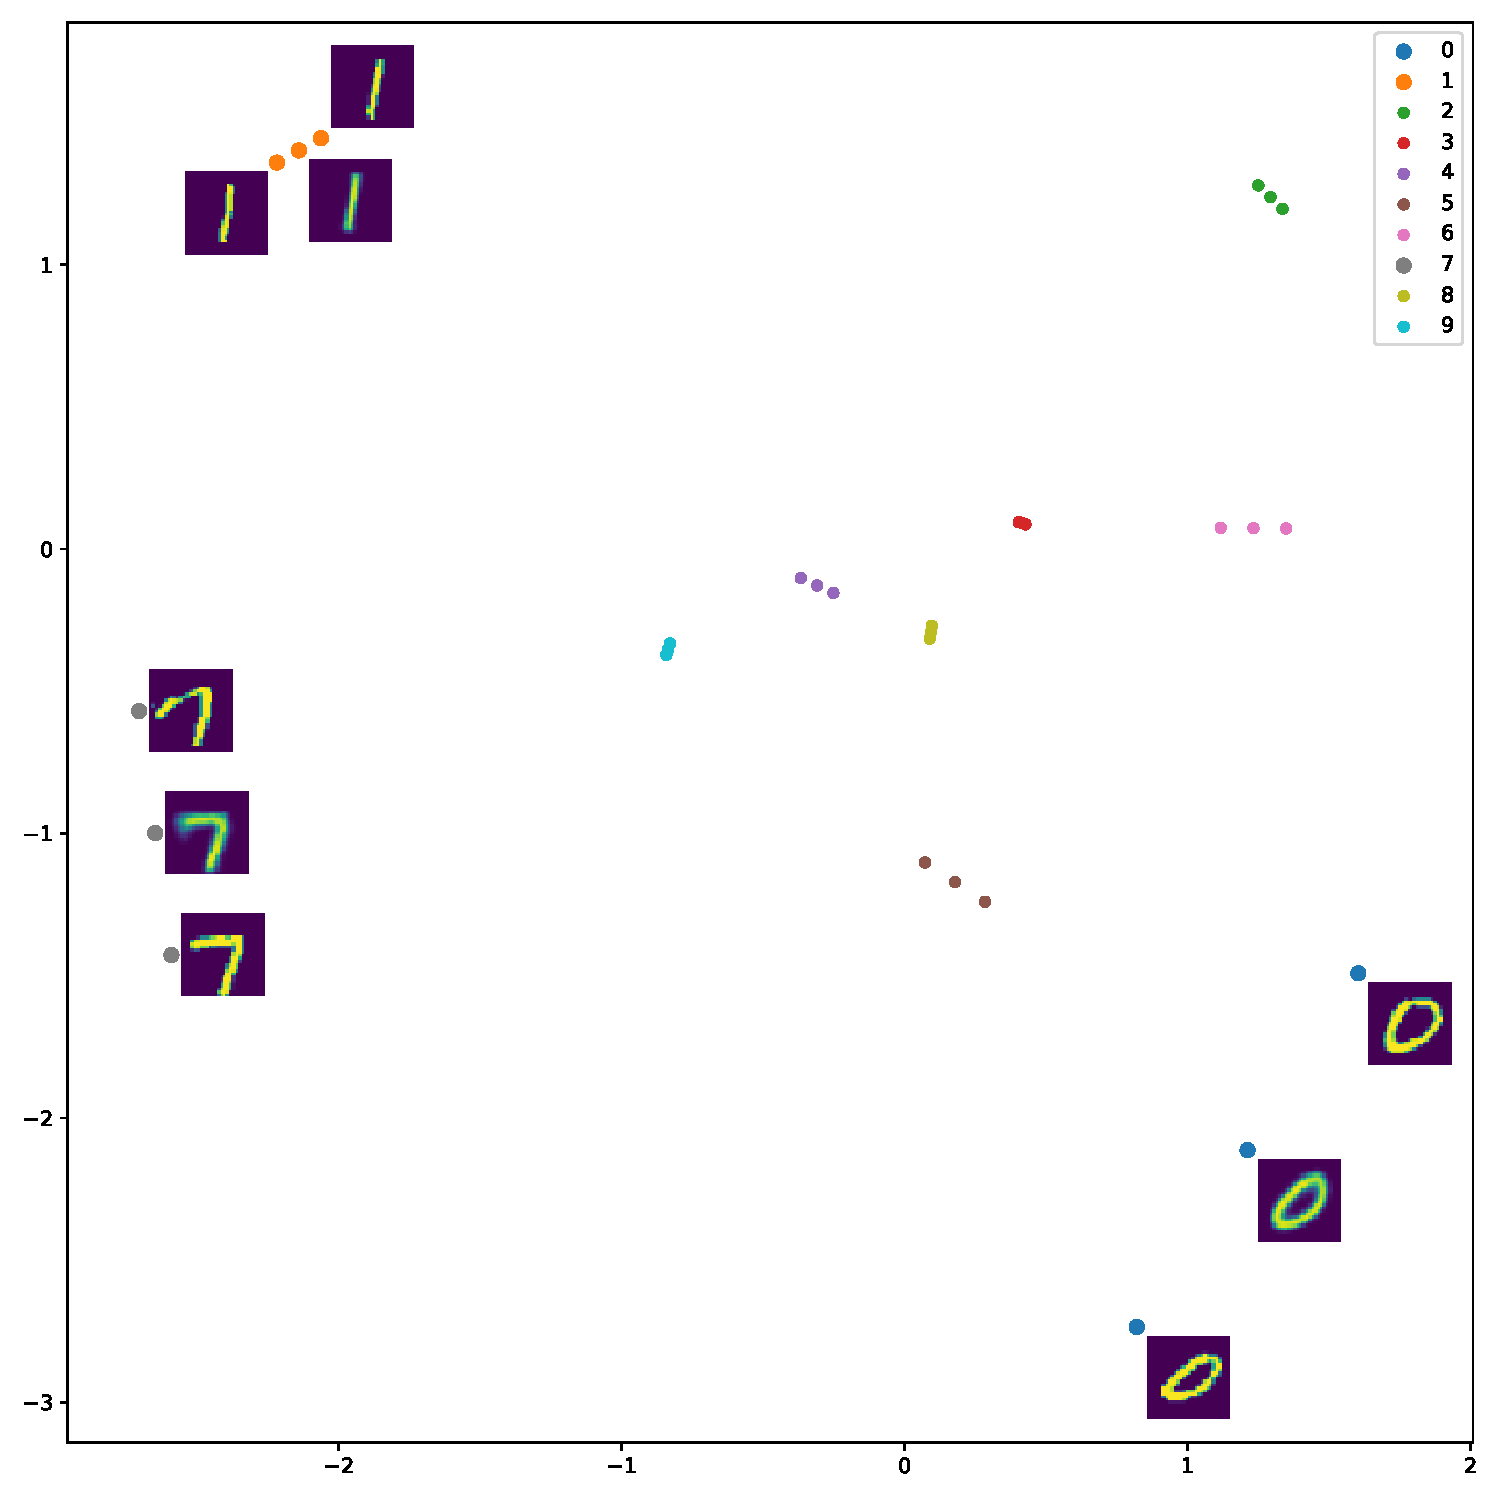
\includegraphics[width=\textwidth]{gfx/evaluation/feature_space/interpolation}
  \caption{Interpolation}
\end{subfigure}%
\begin{subfigure}{.5\textwidth}
  \centering
  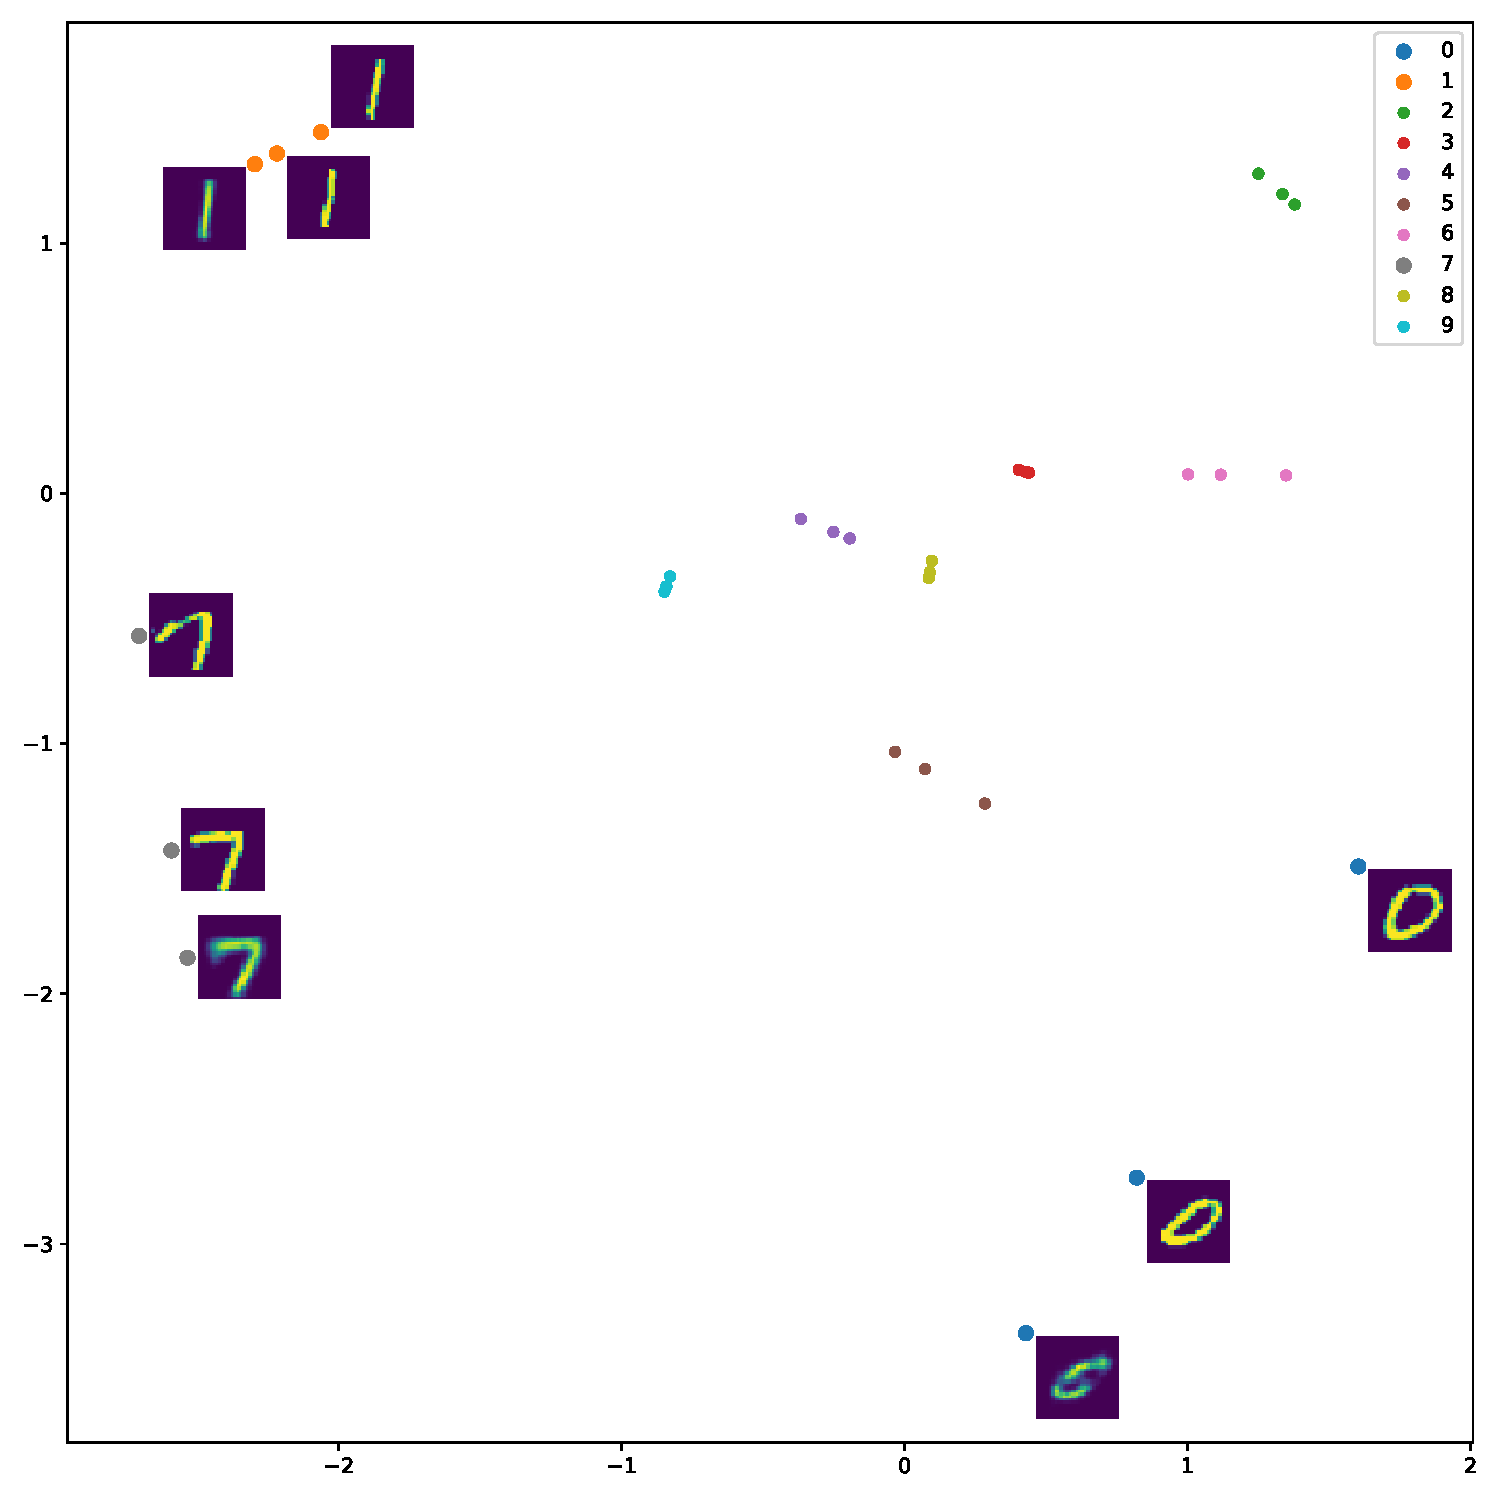
\includegraphics[width=\textwidth]{gfx/evaluation/feature_space/extrapolation}
  \caption{Extrapolation}
\end{subfigure}
\caption{Die Interpolations und Extrapolationsmethode. Zu sehen sind das Ergebnis der nächsten-Nachbar Suche im Latent-Space und der inter- / extrapolierte Punkt für jeweils ein Beispiel jeder Klasse. Der $\alpha$ Parameter wurde auf $0.5$ gesetzt, was bei einer Interpolation genau dem Mittelpunkt entspricht. Zusätzlich sind die Rekonstruktionen der korrespondierenden Punkte zu sehen.}
\label{fig:extrapolation_feature_space}
\end{figure}

In Abb. \ref{fig:mnist_beta_influence} wird der Einfluss des $\beta$ Faktors in der Fehlerfunktion des VAEs gezeigt. Für kleine $\beta$ Werte  ähnelt die Struktur des Latent-Space weniger einer Standardnormalverteilung. Er hat zwar immernoch eine probabilistische Form, welche durch das Sampling im Training (siehe Reparametrisierungstrick, Abschnitt \ref{sec:reparam_trick}) erreicht wird, die Latent-Vektoren weichen aber immer weiter von einem Erwartungswert 0 ab. Der KL-Term ist also essentiell wichtig, um eine bekannte Struktur im Latent-Space zu erzeugen. Gleichzeitig kann eine zu große Gewichtung dazu führen, dass der Latent-Space kollabiert und alle Eingaben auf Erwartungswert 0 und Varianz 1 abbildet. Für Datensätze mit eindeutigen Klassen ist dies von großem Nachteil, da die Merkmale nun voneinander entkoppelt sind (\textit{Disentanglement}, siehe \cite{Higgins2017}). Der Latent-Vektor verliert die Informationen über seine eindeutigen Merkmale. Für Multi-Label Klassifikation kann sich diese Eigenschaft jedoch zu Nutze gemacht werden, um gezielt Merkmale zu dekorrelieren. In den Rekonstruktionen in Abb. \ref{fig:mnist_recon_beta_influence} sehen wir, dass eine größere Gewichtung der KL-Divergenz ein verschwommenere Rekonstruktion mit sich bringt.
%\begin{figure}[H]
%  \centering
%  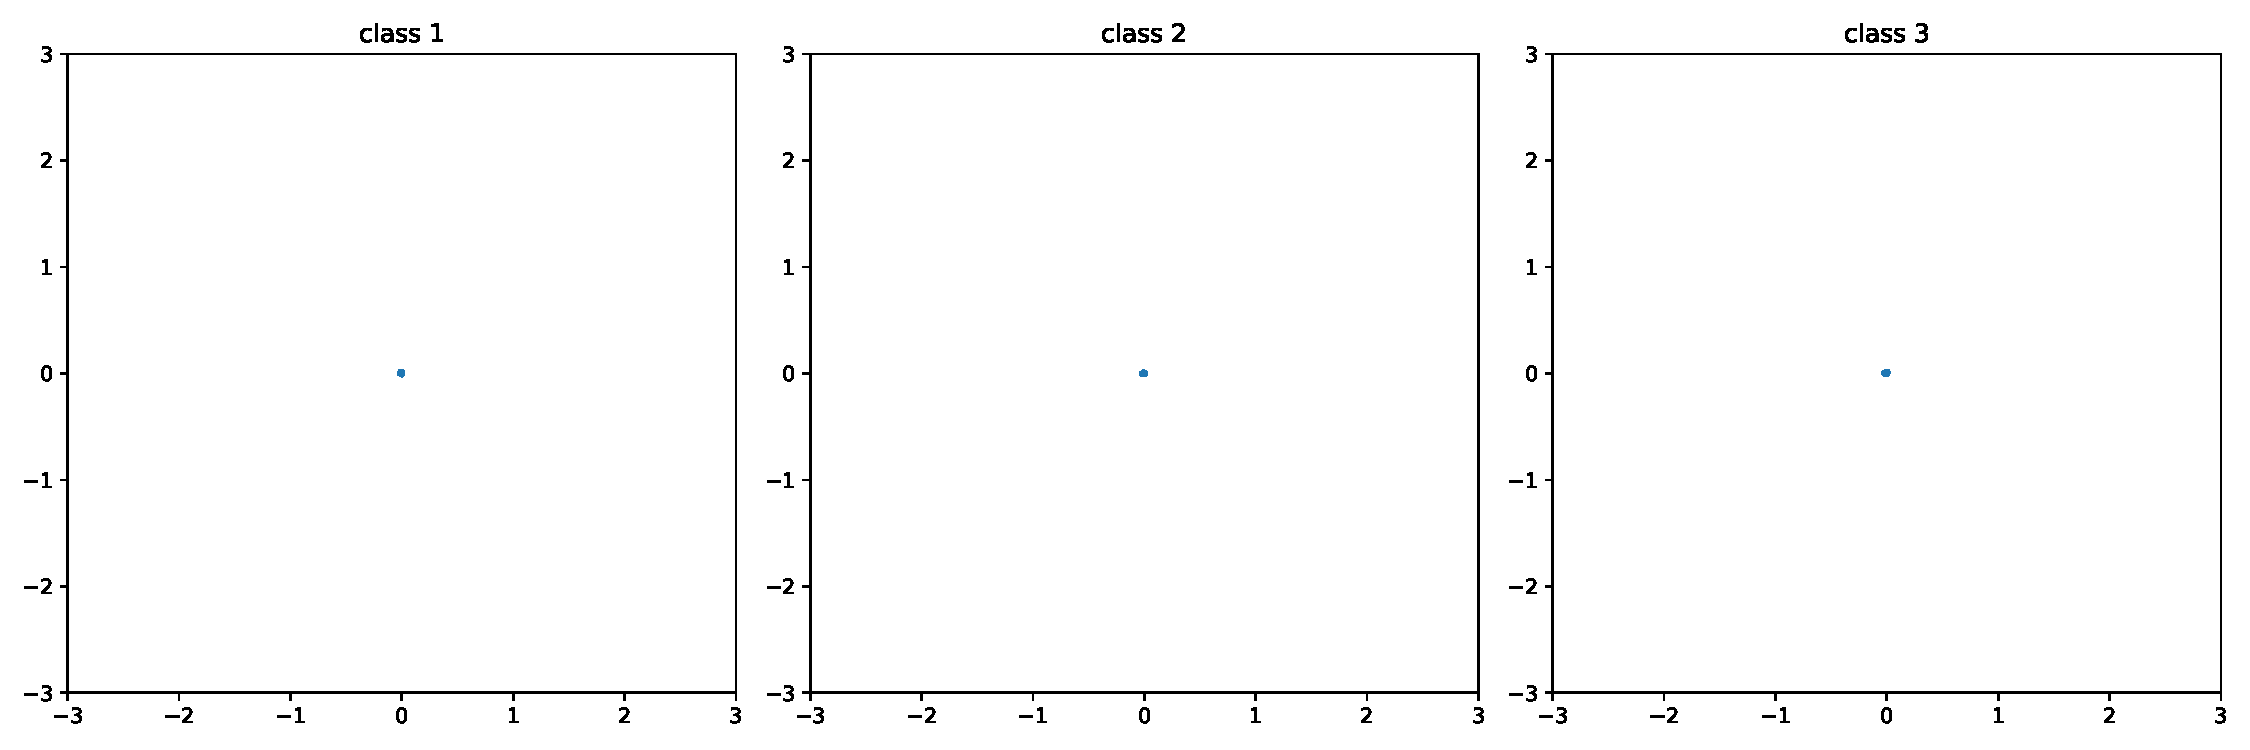
\includegraphics[width=.7\textwidth]{gfx/evaluation/feature_space/thyroid_collapse}
%  \caption{Latent-Space der klassenweisen Multi-VAEs auf dem "thyroid" Datensatzes mit $\beta=1.0$. Alle Eingabebeispiele werden auf den Latent-Vektor 0 abgebildet.}
%  \label{fig:thyroid_collapse}
%\end{figure}

\begin{figure}[H]
\centering
\begin{subfigure}{.28\textwidth}
  \centering
  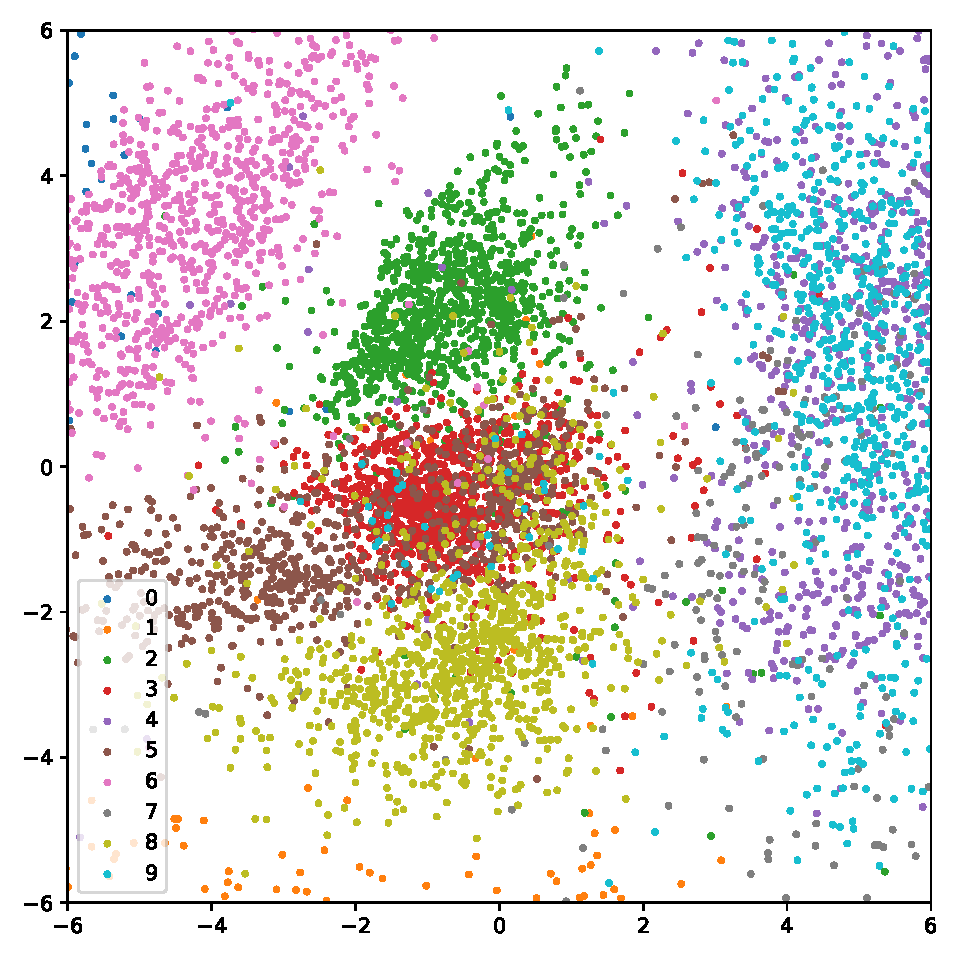
\includegraphics[width=\textwidth]{gfx/evaluation/feature_space/beta=0.001.pdf}
  \caption{$\beta = 0.001$}
\end{subfigure}
\begin{subfigure}{.28\textwidth}
  \centering
  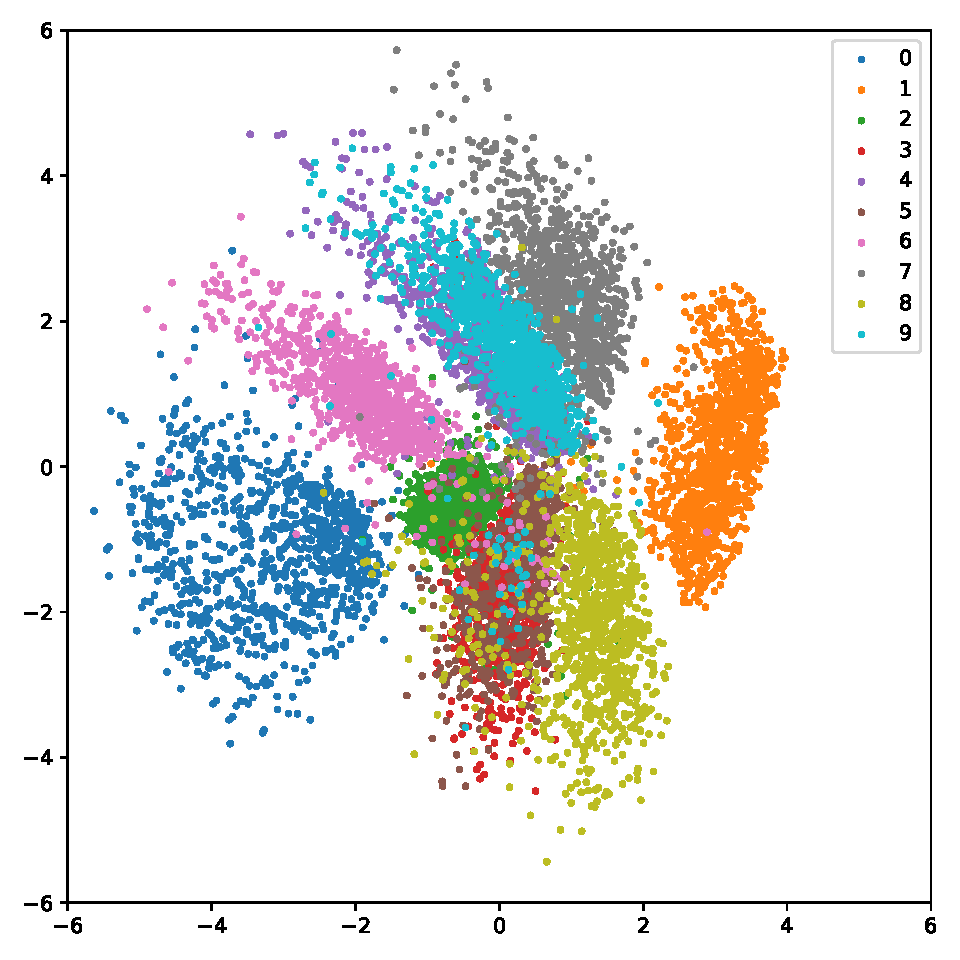
\includegraphics[width=\textwidth]{gfx/evaluation/feature_space/beta=0.1.pdf}
  \caption{$\beta = 0.1$}
\end{subfigure}
\begin{subfigure}{.28\textwidth}
  \centering
  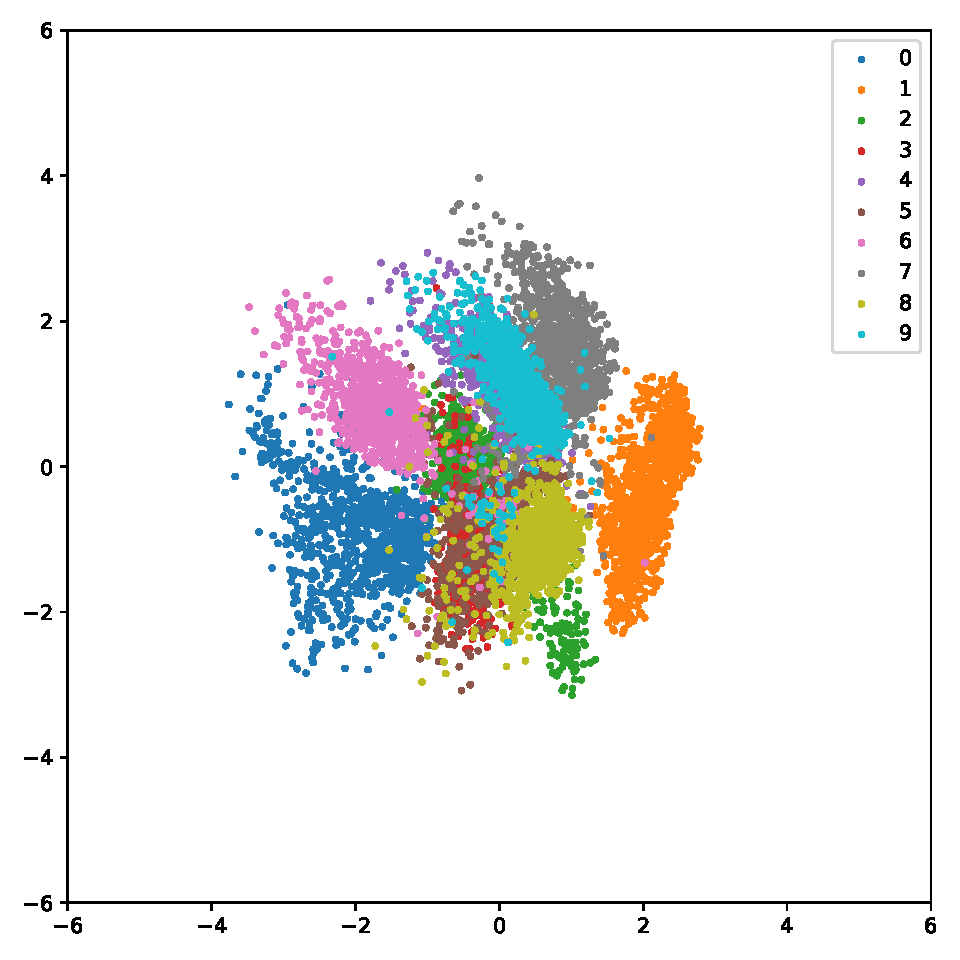
\includegraphics[width=\textwidth]{gfx/evaluation/feature_space/beta=0.5.pdf}
  \caption{$\beta = 0.5$}
\end{subfigure}
\begin{subfigure}{.28\textwidth}
  \centering
  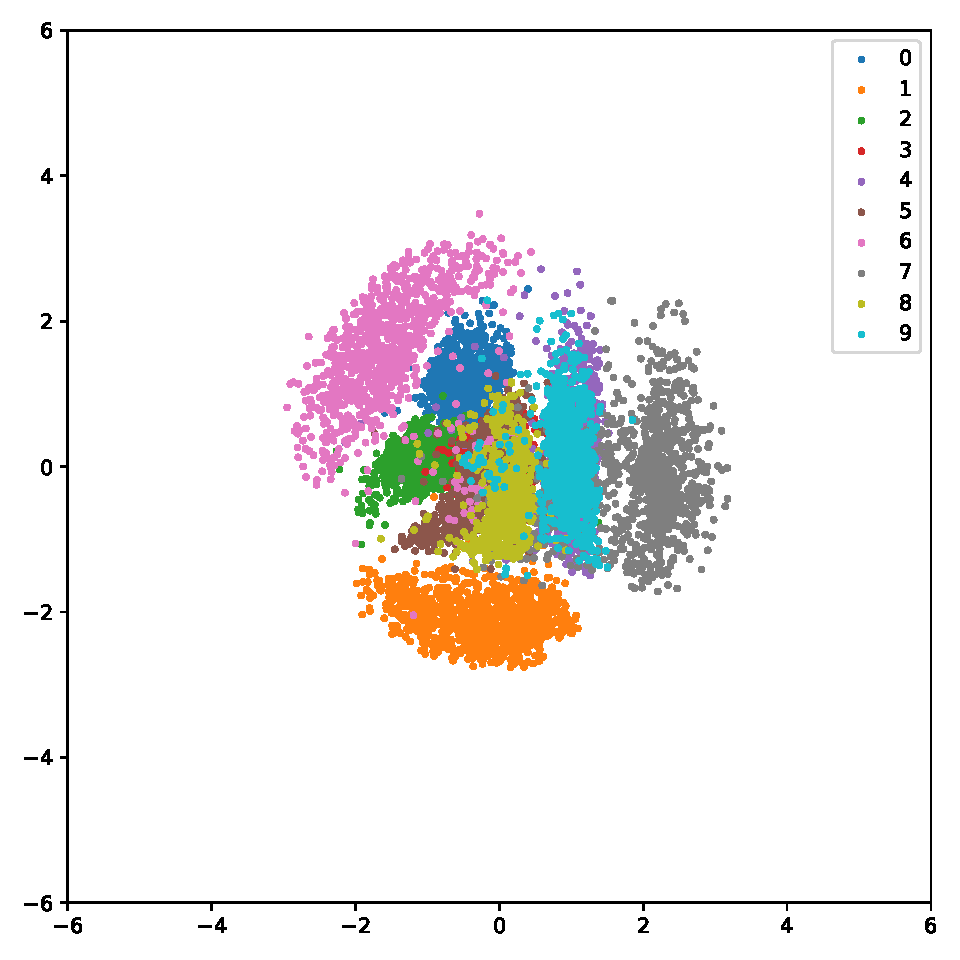
\includegraphics[width=\textwidth]{gfx/evaluation/feature_space/beta=1.0.pdf}
  \caption{$\beta = 1.0$}
\end{subfigure}
\begin{subfigure}{.28\textwidth}
  \centering
  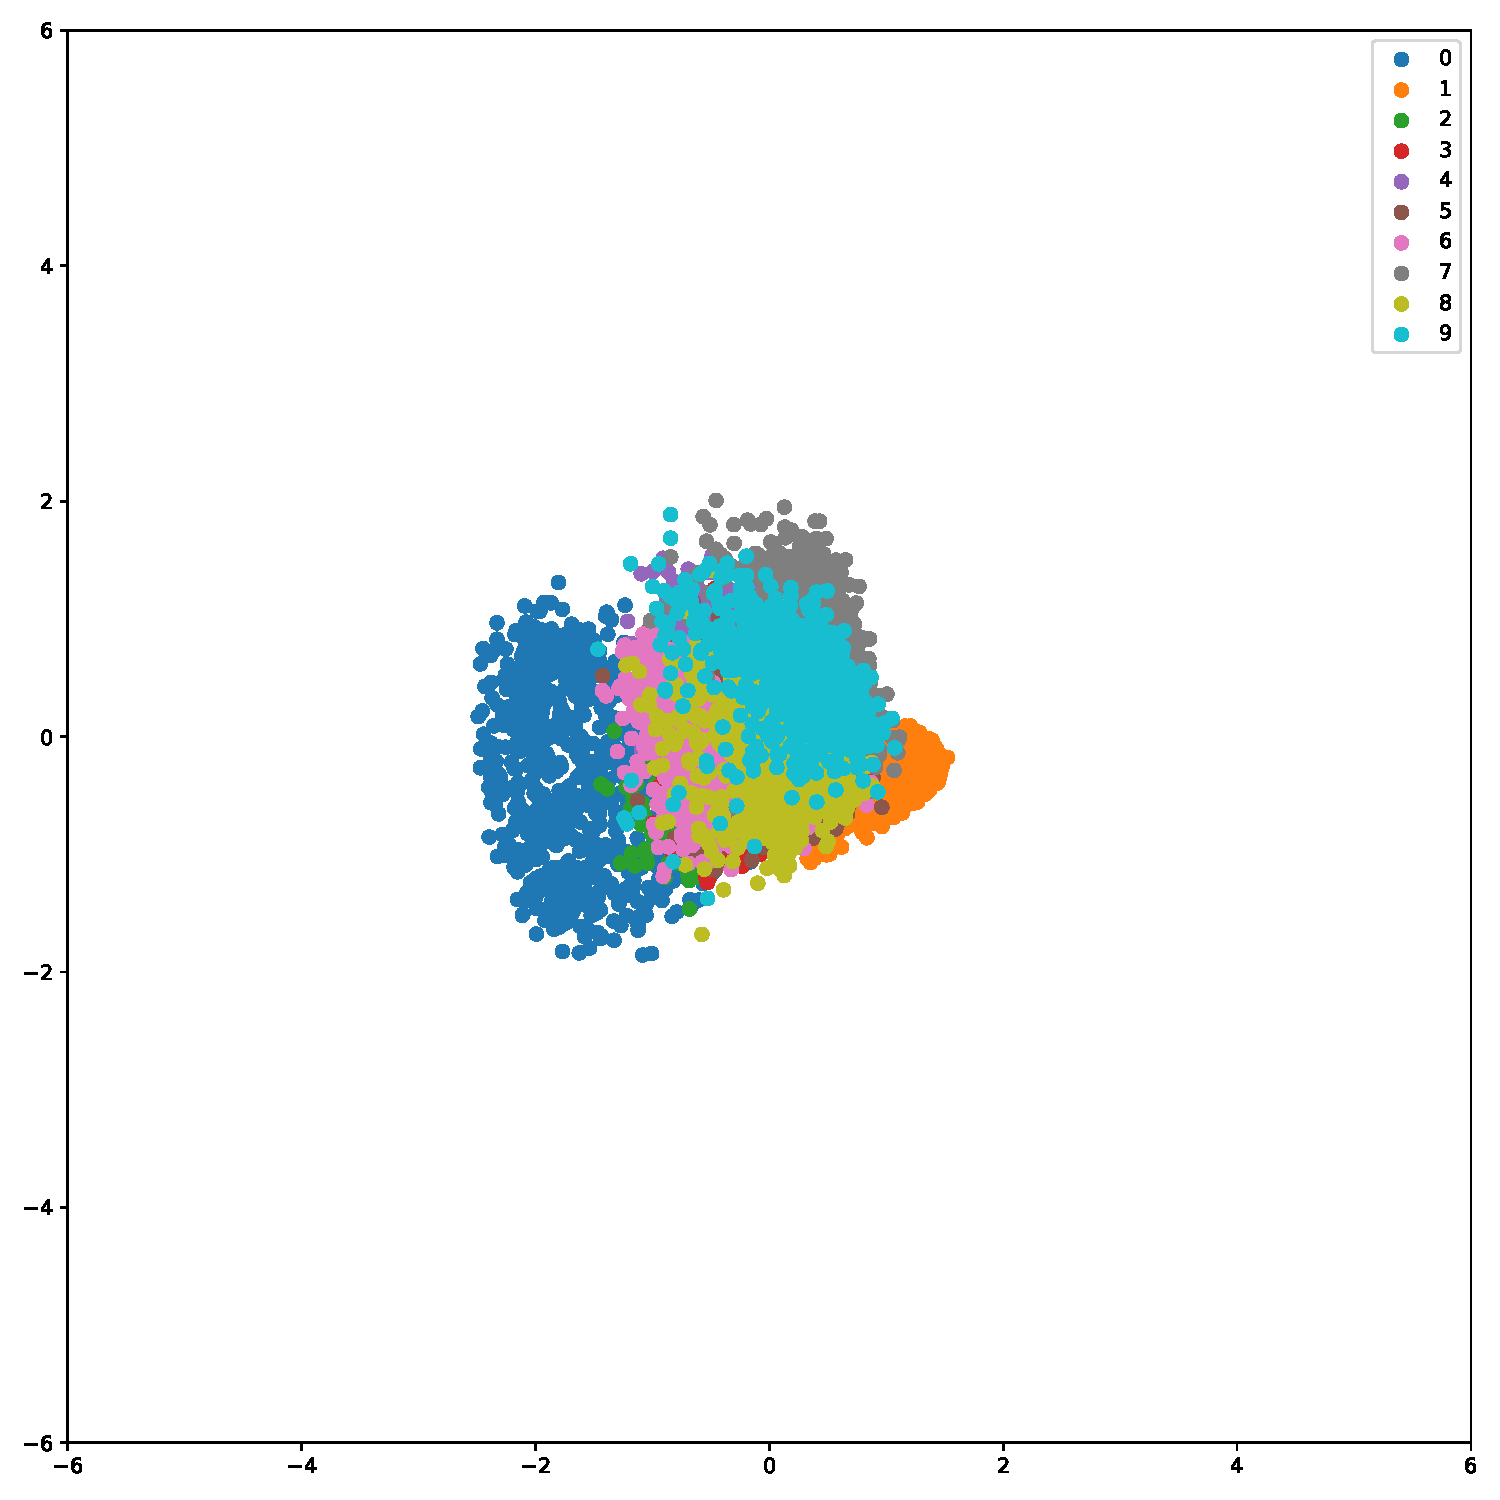
\includegraphics[width=\textwidth]{gfx/evaluation/feature_space/beta=10.0.pdf}
  \caption{$\beta = 10.0$}
\end{subfigure}
\caption{Der Latent-Space eines Single-VAEs (MNIST) für verschiedene Werte von $\beta$. Erkennbar ist, dass zu kleine Werte für $\beta$ weniger Annahmen über die Latent-Vektoren ermöglichen. Zu große Werte haben dagegen einen vollständigen Strukturverlust zur Folge.}
\label{fig:mnist_beta_influence}
\end{figure}

\begin{figure}[H]
  \centering
  
\includegraphics[width=1.3\textwidth]{gfx/evaluation/feature_space/mnist_beta=50.0}
  
\includegraphics[width=1.3\textwidth]{gfx/evaluation/feature_space/mnist_beta=1.0}
  
\includegraphics[width=1.3\textwidth]{gfx/evaluation/feature_space/mnist_beta=norm}
  \caption{Rekonstruktionen zufälliger MNIST Beispiele eines Single-VAEs. Höhere Werte für $\beta$ haben deutlich unschärfere rekonstruierte Bilder zur Folge. Extrem kleine Werte beeinträchtigen die Rekonstruktionsqualität dagegen nicht.}
  \label{fig:mnist_recon_beta_influence}
\end{figure}

Für numerische Daten in den PROBEN1 Datensätzen hat es sich als außerordentlich schwierig erwiesen, geeignete Hyperparameter für einen strukturierten Latent-Space zu finden. In vielen Fällen kollabierte der Latent-Space schon für Werte für $\beta > 0.5$. Ein Grund dafür ist das Verhältnis des BCE-Fehlers zur KL-Divergenz. Für MNIST ist der BCE-Fehler entsprechend groß, da die Bildgröße mit $28 \times 28$ Pixeln einen hohen BCE-Fehler bewirkt (vgl. Reduktion des BCE-Fehlers, Abschnitt \ref{sec:beta_vae}). Im Falle von PROBEN1 jedoch ist die Eingabe nur 8-60 dimensional. Über $\beta$-Normalisierung konnte diesem Problem in den meisten Fällen entgegen gewirkt werden. Bei numerischen Daten hatten auch Batch-Größen von über 32 einen negativen Effekt auf die Struktur des Latent-Spaces. \\

Ein weiteres Problem bei den numerischen Daten des PROBEN1 Datensatzes sind die diskreten Attribute. In Abb. \ref{fig:discrete_problem} ist eine Clusterbildung im Latent-Space zu erkennen.
\begin{figure}[H]
  \centering
  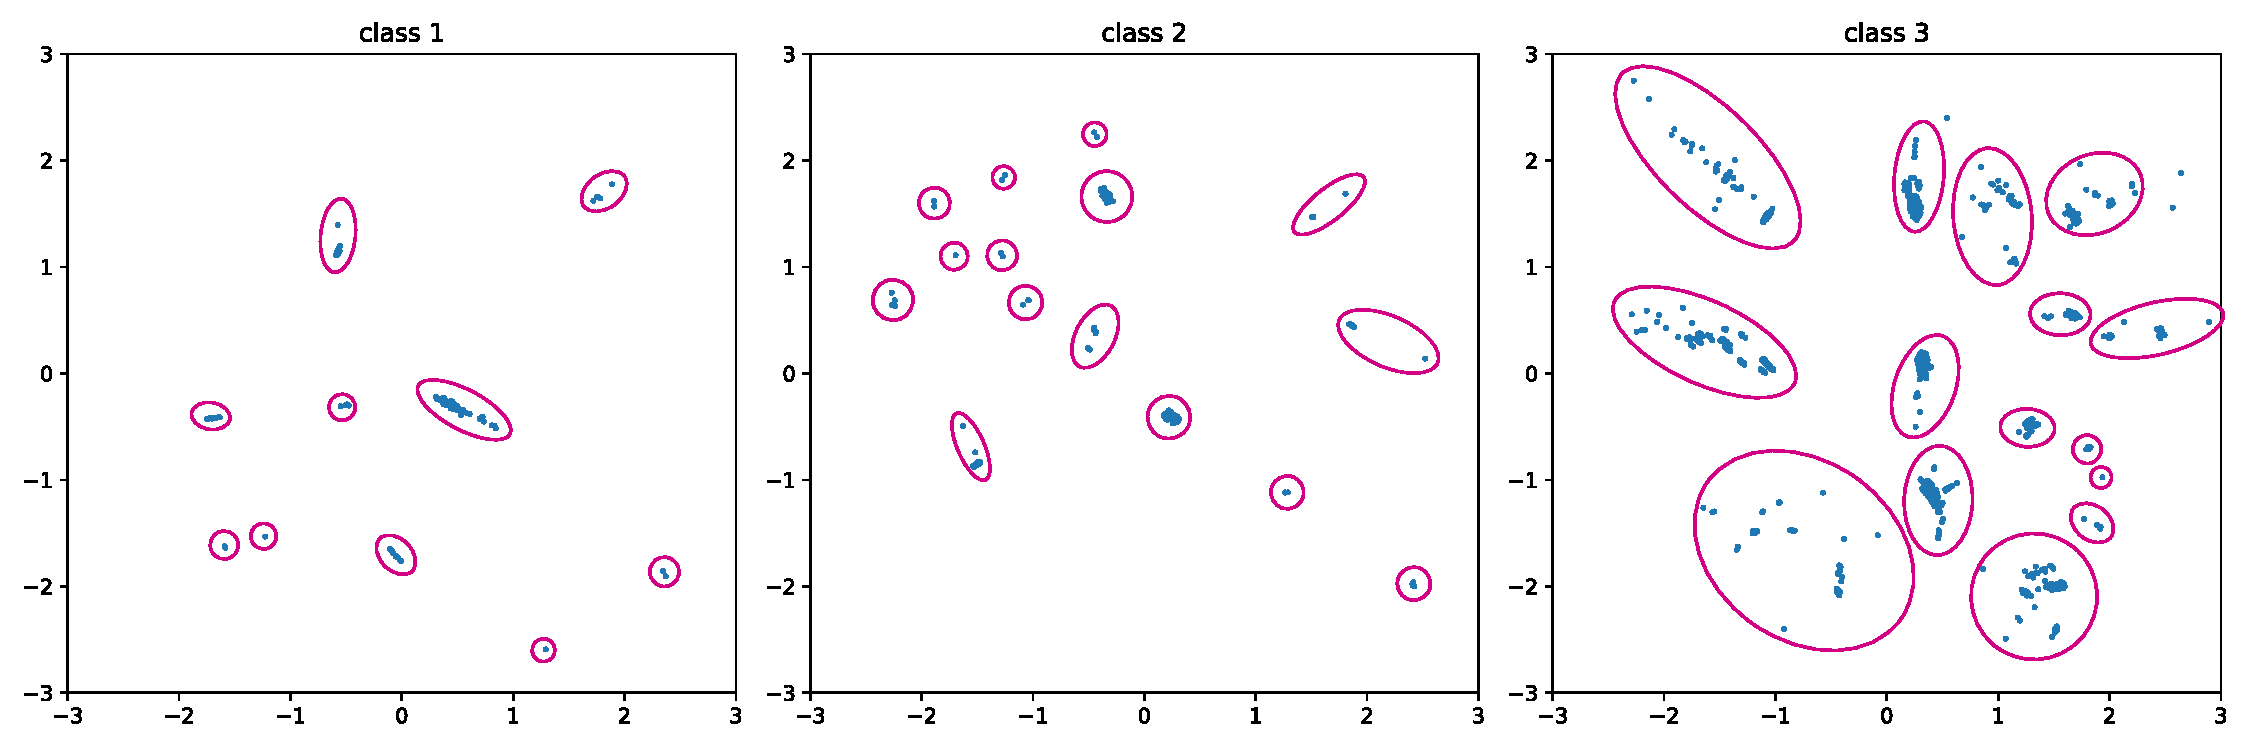
\includegraphics[width=\textwidth]{gfx/evaluation/feature_space/discrete_problem_with_cluster}
  \caption{Latent-Spaces der Klassenweisen VAEs auf dem "thyroid" Datensatz. Der Datensatz besitzt 15 diskrete Attribute und 6 kontinuierliche Attribute. Besonders im Latent-Space zur Klasse 2 führen diese 15 diskreten Attribute zu 15 Clustern.}
  \label{fig:discrete_problem}
\end{figure}
Es zeigt sich eine Relation zwischen der Anzahl an diskreten Attributen und Clustern. Für jedes Attribut entsteht ein Teil-Cluster für jeden Wert aus dem Wertebereich des Attributes. In der Abbildung ist dies besonders in Klasse 2 zu sehen. Man beachte, dass die Attribute des Datensatzes "thyroid" alle binär sind, also 2 Teil-Cluster erkennbar sind. Im Latent-Space der Klasse 3 ist dieses Clustering weniger scharf, aber ebenfalls erkennbar. Grund hierfür ist, dass die Klasse 3 insgesamt 5333 Beispiele, die Klasse 2 dagegen nur 294 Beispiele enthält. So wird der Zwischenraum innerhalb der Cluster in Klasse 3 mehr exploriert. Dieses Clustering ist problematisch für das Generieren neuer Beispiele. Die Grundannahme für das Sampling im Latent-Space besteht darin, dass die Verteilung ähnlich zu einer Standard Normalverteilung ist. Erzielt die KL-Divergenz Regularisierung diese Struktur nicht, so werden Rekonstruktionen erzeugt, welche stark verrauscht sind. Dies hat einen negativen Einfluss auf das Training eines Klassifikators auf diesen generierten Daten.




\section{PROBEN1}
Die Experimente auf den PROBEN1 Datensätzen stellten sich als sehr Hyperparameter sensitiv heraus. So hatte beispielsweise der $\beta$ Parameter, die Batch-Größe des VAEs und die Trainingsdauer des VAEs einen erheblichen Einfluss auf die Resultate. Eine Erkenntnis war, dass die Gefahr des Overfittings beim VAE relativ gering ist. Generell galt: Je länger der VAE trainiert wurde, desto besser wurden die Rekonstruktionen und damit die Ergebnisse im Training mit generierten Daten. Ab ca. 6000 Trainingsschritten (je nach Größe des Datensatzes), verbessert sich die Qualität der Rekonstruktionen nicht mehr. Dies ist nicht überraschend, da Regularisierung des KL-Terms und das Sampling während des Trainings Overfitting verhindern.
In den Experimenten zu PROBEN1 wurde sowohl der Multi-VAE, als auch Single-VAE auf der selben Datenmenge trainiert. Hierbei stellte sich heraus, dass sowohl auf dem gesamten Datensatz, als auch im Few-Shot Szenario der Single-VAE Ansatz keine Verbesserung in der Klassifikation erzielen konnte. Grund dafür ist dass die Eigenschaft des selbst-überwachten Lernens nicht durch zusätzliche nicht-annotierte Daten ausgenutzt werden kann. Ebenso übertraf das zufällige Sampling aus der Normalverteilung $\cN(0, 1)$ die anderen Sampling Methoden im Multi-VAE Fall. Die hier beschriebenen Ergebnisse beschränken sich daher auf den Multi-VAE Ansatz mit Sampling aus der Standardnormalverteilung.

\subsection{Performanz auf dem gesamtem Datensatz}
Für das Training eines Klassifikators auf jeweils dem gesamten Datensatz konnten Verbesserungen des \textit{weighted-f-score} in fast allen Datensätzen erzielt werden. Für das Training mit generierten Daten wurden genauso viele echte Trainingsbeispiele wie generierte benutzt. Mehr generierte Daten hinzuzunehmen, erzielte auf diesen Datensätze keine Verbesserungen. Die Anzahl an Trainingsschritten für den VAE und die Sensitivität des Generative Classifiers wurde jeweils an den Datensatz angepasst. Alle VAEs wurden mit Latent-Space Dimension $d = 2$ trainiert. Es stellte sich heraus, dass eine höhere Dimension auf diesen Datensätzen keine Verbesserung zur Folge hatte. Abb. \ref{tab:eval_proben1_all} zeigt den \textit{weighted-f-score} des Klassifikationsnetzwerks auf den Originaldaten (Baseline), den generierten Daten (VAE) und den gefilterten Daten des Generative Classifiers (VAE + GC). \\

Es ist eine leichte Verbesserung des F-Scores für die mit VAE Daten trainierten Modelle sichtbar. Die höchste Verbesserung konnte im Datensatz "horse" mit 0.016 erzielt werden. Die Datensätze "thyroid" und "geneN" erreichten eine Verbesserung nur, wenn kein Balancing erfolgte. Das Mischen der klassenweisen Datensätze führte hierbei zu einem höheren F-Score. In den anderen Datensätzen konnten bessere Ergebnisse erzielt werden, wenn nicht gemischt, dafür aber die kleineren Klassen ausbalanciert wurden. Die identischen F-Score Werte für den Datensatz "glass" lassen sich dadurch begründen, dass der F-Score für 2 der 3 Seeds bei $1.00$ lag, die Baseline also bereits nahezu fehlerfrei war. Generell ist die Verbesserung mit generierten Daten sehr gering und hängt stark vom Datensatz und der Wahl des Seeds ab. Es ist nicht auszuschließen, dass Zufalls Effekte hier eine Rolle spielen. imbalancierte Datensätze wie "thyroid" erzielen tendenziell weniger Verbesserungen mit dem VAE Ansatz. Der Generative Classifier führt in einigen Fällen zu einem höheren F-Score als der VAE ohne GC. Jedoch fiel beim Trainieren auf, dass je nach Seed die Sensitivität für "schlechte" Beispiele unterschiedlich hoch war. Seed übergreifend Hyperparameter zu finden, erwies sich als äußerst schwierig. \\

Im Vergleich zu den generativen Modellen der Autoren \cite{Moreno-Barea2020} liefert der hier verwendete VAE Ansatz eine geringere Modellgüte. Insbesondere die dort verwendeten Generative-Adversarial-Networks erzielten bessere Resultate.

\begin{table}[hbt]
\centering
\scalebox{.8}{\begin{tabular}{l|c|c|c|c}
\toprule
Datensatz      & $\beta$             & Baseline & VAE            & VAE + GC       \\ \hline
card           & norm=0.133          & 0.871    & 0.873          & 0.869          \\
balance: Ja    & 0.5                 & 0.871    & 0.868          & 0.864          \\
Mix data: Nein & \textbf{1.0}        & 0.871    & \textbf{0.876} & 0.871          \\ \midrule
diabetes       & norm=0.25           & 0.823    & 0.831          & 0.826          \\
balance: Ja    & 0.5                 & 0.823    & 0.830          & 0.822          \\
Mix data: Nein & \textbf{1.0}        & 0.823    & 0.827          & \textbf{0.833} \\ \midrule
geneN          & norm=0.033          & 0.813    & 0.802          & 0.814          \\
balance: Nein  & \textbf{0.5}        & 0.813    & \textbf{0.818} & 0.813          \\
Mix data: Ja   & 1.0                 & 0.813    & 0.812          & 0.813          \\ \midrule
glass          & norm=0.222          & 0.985    & 0.977          & 0.985          \\
balance: Ja    & 0.5                 & 0.985    & 0.977          & 0.985          \\
Mix data: Nein & 1.0                 & 0.985    & 0.984          & 0.985          \\ \midrule
horse          & \textbf{norm=0.1}   & 0.828    & 0.837          & \textbf{0.844} \\
balance: Ja    & 0.5                 & 0.828    & 0.833          & 0.835          \\
Mix data: Nein & 1.0                 & 0.828    & 0.836          & 0.828          \\ \midrule
thyroid        & \textbf{norm=0.095} & 0.954    & 0.952          & \textbf{0.956} \\
balance: Nein  & \textbf{0.5}        & 0.954    & 0.927          & \textbf{0.956} \\
Mix data: Ja   & 1.0                 & 0.954    & 0.925          & 0.954          \\
\bottomrule
\end{tabular}}
\caption{F-Scores auf den PROBEN1 Datensätzen. Das beste Ergebnis ist jeweils \textbf{fett} gedruckt. Bis auf den "glass" Datensatz verbessert sich der F-Score durch den VAE um ca. $0.007$. Es wurden 3 verschiedene Werte für $\beta$ getestet: $1.0, 0.5$ und $1.0$ mit $\beta$-Normalisation (mit norm angegeben). Höhere Werte für $\beta$ führten zum Kollaps im Latent-Space und daraus resultierend schlechterer Güte.}
\label{tab:eval_proben1_all}
\end{table}


\subsection{Few-Shot Szenario}
Abbildung \ref{plt:thyroid-few-shot} zeigt, dass die Verbesserung im F-Score mit zunehmender Anzahl an Trainingsbeispielen abnimmt. Ab 50 Beispielen pro Klasse ist sogar keine Verbesserung mehr sichtbar. Der Baseline Score liegt dann schon entsprechend hoch. Es scheint, als würden die verrauschten Beispiele, die der VAE generiert, die Klassifikationsaufgabe erschweren. Lediglich bei sehr wenig Beispielen pro Klasse sind die Beispiele hilfreich für die Klassifikation. Der Generative Classifier scheint das Ergebnis nicht konsequent zu verbessern.

\begin{table}[H]
\centering
\scalebox{.8}{\begin{tabular}{l|l|c|c|c}
\toprule
\# Trainingsbeispiele & \# Generierte Beispiele & Baseline       & VAE            & VAE + GC       \\ \hline
5                     & 5                       & 0.619          & \textbf{0.693} & 0.675          \\
10                    & 10                      & 0.727          & \textbf{0.778} & 0.761          \\
20                    & 20                      & 0.735          & 0.753          & \textbf{0.778} \\
30                    & 30                      & 0.772          & 0.786          & \textbf{0.796} \\
50                    & 50                      & \textbf{0.818} & 0.815          & 0.808          \\
100                   & 100                     & \textbf{0.935} & 0.927          & 0.922          \\
\bottomrule
\end{tabular}}
\caption{Der F-Score auf dem Datensatz "thyroid" im Few-Shot Szenario. Für kleine Trainingsgrößen ergibt sich ein verbesserte Wert von bis zu $0.074$. Die Verbesserung nimmt mit der Anzahl originaler Trainingsbeispiele ab.}
\label{tab:eval_thyroid_few_shot}
\end{table}

\begin{figure}[H]
\centering
\begin{tikzpicture}
\begin{axis}
[
  width=.6\textwidth,
  height = 4cm,
  symbolic x coords={5,10,20,30,50,100},
  xtick={5,10,20,30,50,100},
  xlabel={\# Beispiele pro Klasse}, 
  ylabel={$\Delta$ F-Score}, 
  grid,
  legend pos=south west,
]

\addplot[blue, mark=* , solid] table[col sep=comma, x=n_originals, y=improvement]{data/evaluation/thyroid-few-shot.csv};
\addlegendentry{F1-Increase}

\end{axis}
\end{tikzpicture}
\caption{Differenz des Baseline F-Scores und des Multi-VAEs auf dem Datensatz "thyroid" im Few-Shot-Szenario. Es wurde jeweils der höchste Wert von VAE und VAE + GC verwendet}
\label{plt:thyroid-few-shot}
\end{figure}

%\begin{table}[hbt]
%\centering
%\begin{tabular}{l|l|c|c|c}
%\toprule
%\# Trainingsbeispiele & \# Generierte Beispiele & Baseline       & VAE            & VAE + GC       \\ \hline
%2                     & 2                       & \textbf{0.657} & 0.652          & 0.652          \\
%3                     & 3                       & 0.782          & \textbf{0.788} & 0.756          \\
%4                     & 4                       & 0.748          & 0.753          & \textbf{0.758} \\
%5                     & 5                       & \textbf{0.740} & 0.721          & 0.724          \\
%10                    & 10                      & 0.731          & 0.729          & \textbf{0.763} \\
%20                    & 20                      & 0.803          & 0.783          & \textbf{0.816} \\
%30                    & 30                      & 0.853          & 0.870          & \textbf{0.871} \\
%50                    & 50                      & 0.854          & 0.854          & \textbf{0.862} \\
%100                   & 100                     & \textbf{0.867} & 0.857          & \textbf{0.867} \\
%200                   & 200                     & 0.879          & 0.882          & \textbf{0.883} \\
%500                   & 500                     & 0.879          & 0.874          & \textbf{0.888} \\
%1000                  & 1000                    & 0.879          & \textbf{0.883} & 0.879          \\
%2000                  & 2000                    & \textbf{0.879} & 0.874          & 0.874          \\
%\bottomrule
%\end{tabular}
%\caption{Evaluation des Datensatzes horse in einem Few-Shot Szenario.}
%\label{tab:eval_horse_few_shot}
%\end{}

\section{MNIST}
In unseren Experimenten zum MNIST Datensatz wurden die klassenweisen VAEs für den Multi-VAE Ansatz stets auf der angegebenen Menge an Beispielen pro Klasse trainiert. Als Latent-Space Dimension wurde $d = 2$ gewählt und die KL-Divergenz wurde mit $\beta = 0.5$ gewichtet, um schärfere Bilder zu generieren. Die Multi-VAE Modelle wurden alle für 6000 Schritte trainiert. Für den Single-VAE Ansatz wurde ein Modell selbst-überwacht auf dem gesamten Trainingsdatensatz (60000 Bilder) trainiert. Die Latent-Space Dimension dieses Modells wurde auf $d = 50$ gesetzt. Der $\beta$ Faktor lag bei $1.0$. Das verwendete Modell wurde für 93 000 Schritte trainiert. Die Trainingszeit lag bei $\approx 15 min$. Da die Klassifikation des MNIST Datensatzes mit 60000 Trainingsbeispielen als gelöstes Problem gilt, wird dieser Fall nicht betrachtet. Untersuchen jedoch zusätzlich zum Few-Shot Fall das Training auf nur generierten Daten des VAEs. In allen Experimenten zum MNIST Datensatz wurden dieselben Seeds verwendet.

\subsection{Few-Shot Szenario}\label{sec:mnist_few_shot}
Für das Few-Shot Szenario wurden die in Abschnitt \ref{sec:sampling} beschriebenen Generationsmethoden für den Single-VAE sowie das Sampling aus einer Standardnormalverteilung für den Multi-VAE Ansatz evaluiert. Ebenso wurden diese Methoden mit und ohne Generative Classifier betrachtet. Tabelle \ref{tab:mnist_few_shot} zeigt die Güte der verschiedenen Ansätze für unterschiedliche Trainingsgrößen. Für dieses Experiment wurden original Beispiele und Generierte im Verhältnis 1:1 verwendet.
\begin{table}[hbt]
\centering
\scalebox{.8}{\begin{tabular}{l|c|c|c|c|c|c|c}
\toprule
\begin{tabular}[c]{@{}l@{}}\# Beispiele\\ pro Klasse\end{tabular} & Baseline       & Noise & Interpolation  & Extrapolation  & \begin{tabular}[c]{@{}c@{}}Interpolation\\ + Noise\end{tabular} & \begin{tabular}[c]{@{}c@{}}Extrapolation\\ + Noise\end{tabular} & Multi-VAE      \\ \hline
2                                                                 & 0.660          & 0.619 & 0.669          & 0.654          & 0.674                                                           & 0.653                                                           & \textbf{0.678} \\
3                                                                 & 0.699          & 0.662 & \textbf{0.706} & 0.700          & 0.703                                                           & \textbf{0.706}                                                  & \textbf{0.706} \\
4                                                                 & 0.734          & 0.703 & 0.740          & 0.732          & \textbf{0.744}                                                  & 0.734                                                           & 0.734          \\
5                                                                 & 0.776          & 0.721 & 0.782          & 0.756          & \textbf{0.787}                                                  & 0.768                                                           & 0.770          \\
10                                                                & 0.849          & 0.825 & 0.855          & \textbf{0.861} & 0.859                                                           & 0.849                                                           & 0.854          \\
20                                                                & 0.905          & 0.878 & 0.905          & \textbf{0.911} & 0.905                                                           & 0.909                                                           & 0.904          \\
30                                                                & 0.929          & 0.898 & 0.924          & \textbf{0.930} & 0.927                                                           & 0.923                                                           & 0.923          \\
50                                                                & 0.941          & 0.920 & 0.939          & 0.941          & \textbf{0.942}                                                  & 0.938                                                           & 0.937          \\
100                                                               & \textbf{0.954} & 0.940 & 0.951          & 0.953          & 0.951                                                           & 0.950                                                           & 0.949          \\
200                                                               & \textbf{0.962} & 0.950 & 0.958          & 0.960          & 0.956                                                           & 0.958                                                           & 0.956          \\
500                                                               & \textbf{0.964} & 0.955 & 0.962          & 0.963          & 0.962                                                           & 0.963                                                           & 0.959          \\
1000                                                              & \textbf{0.965} & 0.952 & 0.963          & 0.964          & 0.964                                                           & 0.963                                                           & 0.960          \\
2000                                                              & \textbf{0.967} & 0.953 & 0.964          & 0.966          & 0.963                                                           & 0.964                                                           & 0.963          \\
\bottomrule
\end{tabular}}
\caption{Evaluation des Klassifikators auf reduzierten Partitionen des MNIST Datensatzes. Die Werte stellen jeweils das Maximum aus VAE ohne GC und VAE mit GC dar.}
\label{tab:mnist_few_shot}
\end{table}
Zu sehen ist, dass mit zunehmender Datengröße die Verbesserungen durch die generierten Daten abnimmt. Bei mehr als 100 Trainingsbeispielen pro Klasse ist der VAE Ansatz sogar schlechter als die Baseline. Trotzdem verbessert der VAE den F-Score bei wenig Beispielen um bis zu $0.018$. Die Interpolation und Extrapolationsmethoden mit Noise erwiesen sich als die besten Ansätze. Nur Noise lieferte keine Verbesserung. Der Multi-VAE Ansatz zeigt nur im 2-3-Shot Fall eine gute Performance. Im Vergleich zu den Resultaten der Autoren \cite{Garay-Maestre2019} schneidet das hier evaluierte Modell bei höheren Datenmengen schlechter ab. Für über 100 Beispielen pro Klasse konnten die dort erzielten Ergebnisse nicht reproduziert werden. Dies kann aber auch durch das in der vorliegenden Arbeit verwendete Evaluationsverfahren begründet sein, da über 3 unterschiedliche Seeds der Mittelwert gebildet wird.


\subsection{Performanz auf nur generierten Daten}\label{sec:mnist_only_gen}
Da die erzielten Verbesserungen in der Modellgüte gering ausfallen, stellt sich die Frage: Wie mächtig ist der VAE Ansatz? Darum wurden die Resultate des Klassifikators bei einem Training auf nur generierten Daten mit der Baseline verglichen. Ausgangspunkt für das VAE Modell und die Baseline bilden 5 Originalbeispiele. Abb. \ref{plt:mnist_only_gen} zeigt die Entwicklung des F-Scores mit der Zunahme an generierten Beispielen.
\begin{table}[H]
\centering
\scalebox{.8}{\begin{tabular}{l|c|c|c|c|c}
\toprule
\begin{tabular}[c]{@{}l@{}}\# Generierte Beispiele\\ pro Klasse\end{tabular} & Baseline & Noise & \begin{tabular}[c]{@{}c@{}}Interpolation\\ + Noise\end{tabular} & \begin{tabular}[c]{@{}c@{}}Extrapolation\\ + Noise\end{tabular} & Multi-VAE      \\ \hline
2                                                                            & 0.776    & 0.402 & \textbf{0.636}                                                  & 0.542                                                           & 0.635          \\
3                                                                            & 0.776    & 0.518 & \textbf{0.681}                                                  & 0.637                                                           & 0.666          \\
4                                                                            & 0.776    & 0.542 & \textbf{0.699}                                                  & 0.616                                                           & 0.697          \\
5                                                                            & 0.776    & 0.555 & 0.686                                                           & 0.574                                                           & \textbf{0.712} \\
10                                                                           & 0.776    & 0.618 & 0.740                                                           & 0.696                                                           & \textbf{0.764} \\
20                                                                           & 0.776    & 0.670 & 0.748                                                           & 0.740                                                           & \textbf{0.773} \\
30                                                                           & 0.776    & 0.700 & 0.765                                                           & 0.744                                                           & \textbf{0.769} \\
50                                                                           & 0.776    & 0.726 & \textbf{0.774}                                                  & 0.754                                                           & 0.763          \\
100                                                                          & 0.776    & 0.750 & \textbf{0.797}                                                  & 0.771                                                           & 0.768          \\
200                                                                          & 0.776    & 0.765 & \textbf{0.790}                                                  & 0.761                                                           & 0.771          \\
500                                                                          & 0.776    & 0.788 & \textbf{0.792}                                                  & 0.770                                                           & 0.774          \\
1000                                                                         & 0.776    & 0.775 & \textbf{0.788}                                                  & 0.773                                                           & 0.767          \\
2000                                                                         & 0.776    & 0.777 & \textbf{0.792}                                                  & 0.765                                                           & 0.770          \\
\bottomrule
\end{tabular}}
\caption{F-Score bei Training auf ausschließlich generierten Daten. Die Baseline wurde auf 5 Originalbeispielen trainiert. Für den VAE stehen dieselben 5 Beispiele zur Verfügung um Daten zu generieren. Anschließend wurden nur die generierten Daten für die Evaluation der jeweiligen Methode verwendet. Die Methode Interpolation + Noise erzielt insbesondere für viele generierte Beispiele eine hohe Modellgüte, teilweise sogar besser als die Baseline.}
\label{tab:mnist_only_gen}
\end{table}

\begin{figure}[H]
\centering
\begin{tikzpicture}
\begin{axis}
[
  width=.8\textwidth,
  height=5cm,
  symbolic x coords={2,3,4,5,10,20,30,50,100,200,500,1000,2000},
  xtick={2,3,4,5,10,20,30,50,100,200,500,1000,2000},
  xlabel={Generierte Beispiele pro Klasse}, 
  ylabel={F1 Score}, 
  grid,
  legend pos=south east,
]

\addplot[blue, no marks, solid] table[col sep=comma, x=n_generated, y=baseline]{data/evaluation/MNIST-GEN*-5.csv};
\addlegendentry{Baseline}

\addplot[red, no marks, solid] table[col sep=comma, x=n_generated, y=interpolation_noise]{data/evaluation/MNIST-GEN*-5.csv};
\addlegendentry{Interpolation + Noise}

\addplot[violet, no marks, solid] table[col sep=comma, x=n_generated, y=multi_vae]{data/evaluation/MNIST-GEN*-5.csv};
\addlegendentry{Multi-VAE}

\end{axis}
\end{tikzpicture}
\caption{Der Verlauf der Modellgüte bei verschiedenen Mengen von generierten Daten. Die Methode Interpolation + Noise übertrifft die Baseline für eine hohe Anzahl. Die Multi-VAE Methode nähert sich asymptotisch der Baseline Qualität.}
\label{plt:mnist_only_gen}
\end{figure}

Erkennbar ist, dass ab 50 Beispielen die Methode Interpolation mit Noise die Baseline sogar übertrifft. Die Modellgüte nimmt der Anzahl an generierten Beispielen zu.


\subsection{MNIST Few-Shot Szenario - Mehr generierte Daten}
Da Abschnitt \ref{sec:mnist_only_gen} zeigt, dass sich die Modellgüte erhöht, wenn mehr Daten generiert werden, wurde das Few-Shot Szenario zusätzlich mit diesmal 2000 generierten Daten pro Klasse evaluiert. Das Setup ist ansonsten das gleiche wie in Abschnitt \ref{sec:mnist_few_shot}. In Abb. \ref{tab:mnist_2000_gen} ist zu sehen, dass die F-Scores weiter verbessert werden konnten. Der VAE Ansatz erzielt nun einen bis zu 0.022 höheren F-Score als die Baseline. Außerdem zeigt sich, dass die Noise Methode vor allem im 2-4-Shot Fall eine höhere Bewertung erzielt. Für das Multi-VAE Verfahren scheint die Zunahme an generierten Daten kontraproduktiv zu sein.

\begin{table}[hbt]
\centering
\scalebox{.8}{\begin{tabular}{l|c|c|c|c|c}
\toprule
\begin{tabular}[c]{@{}l@{}}\# Beispiele\\ pro Klasse\end{tabular} & Baseline       & Noise          & \begin{tabular}[c]{@{}c@{}}Interpolation\\ + Noise\end{tabular} & \begin{tabular}[c]{@{}c@{}}Extrapolation\\ + Noise\end{tabular} & Multi-VAE \\ \hline
2                                                                 & 0.660          & \textbf{0.679} & 0.668                                                           & 0.638                                                           & 0.634     \\
3                                                                 & 0.699          & \textbf{0.716} & 0.715                                                           & 0.711                                                           & 0.687     \\
4                                                                 & 0.734          & \textbf{0.748} & 0.747                                                           & 0.740                                                           & 0.724     \\
5                                                                 & 0.776          & 0.779          & \textbf{0.795}                                                  & 0.772                                                           & 0.768     \\
10                                                                & 0.849          & 0.851          & 0.868                                                           & \textbf{0.871}                                                  & 0.839     \\
20                                                                & 0.905          & 0.894          & 0.907                                                           & \textbf{0.919}                                                  & 0.897     \\
30                                                                & 0.929          & 0.905          & 0.922                                                           & \textbf{0.936}                                                  & 0.916     \\
50                                                                & 0.941          & 0.914          & 0.935                                                           & \textbf{0.945}                                                  & 0.925     \\
100                                                               & \textbf{0.954} & 0.923          & 0.946                                                           & 0.951                                                           & 0.936     \\
200                                                               & \textbf{0.962} & 0.929          & 0.952                                                           & 0.960                                                           & 0.934     \\
500                                                               & \textbf{0.964} & 0.939          & 0.957                                                           & 0.960                                                           & 0.924     \\
1000                                                              & \textbf{0.965} & 0.946          & 0.960                                                           & 0.961                                                           & 0.913     \\
2000                                                              & \textbf{0.967} & 0.953          & 0.963                                                           & 0.964                                                           & 0.905     \\
\bottomrule
\end{tabular}}
\caption{F-Score auf dem MNIST Datensatz im Few-Shot Szenario. Mit 2000 generierten Beispielen erzielen alle Methoden höhere Werte als bei einer 1:1 Zusammensetzung des Datensatzes.}
\label{tab:mnist_2000_gen}
\end{table}


\section{CelebA}
Die übliche Klassifikationsaufgabe auf dem CelebA Datensatz ist die Multi-Label Klassifikation. Die Aufgabe besteht darin alle Attribute eines Bildobjektes korrekt vorherzusagen. Da dies den Rahmen dieser Arbeit sprengen würde, konzentriert sich unsere Analyse auf Modifikationen im Latent-Space und deren Auswirkung auf die Rekonstruktionen. Da es keine eindeutigen Klassen gibt, wird nur der Single-VAE Ansatz betrachtet. Der Datensatz ist mit ca. 200.000 Bildern  und 10.177 Identitäten sehr groß, daher wurde auch die Latent-Space Dimension mit $d = 50$ entsprechend groß gewählt. Trainiert wurden 2 Modelle mit $\beta$-Normalisation: Eines mit $\beta = 1.0$, das zweite mit $\beta = 150$. In Abb. \ref{fig:celeba_recon} sehen wir, dass die Rekonstruktionen deutlich verrauscht sind. Außerdem ist zu erkennen, dass dies bei $\beta = 150$ stärker der Fall ist. Der hohe $\beta$ Faktor hat also einen negativen Einfluss auf die Qualität der Rekonstruktionen. Der $\beta$ Faktor hat aber auch einen Einfluss auf die Representationen der extrahierten Merkmale im Latent-Space.

\begin{figure}[hbt]
  \centering
  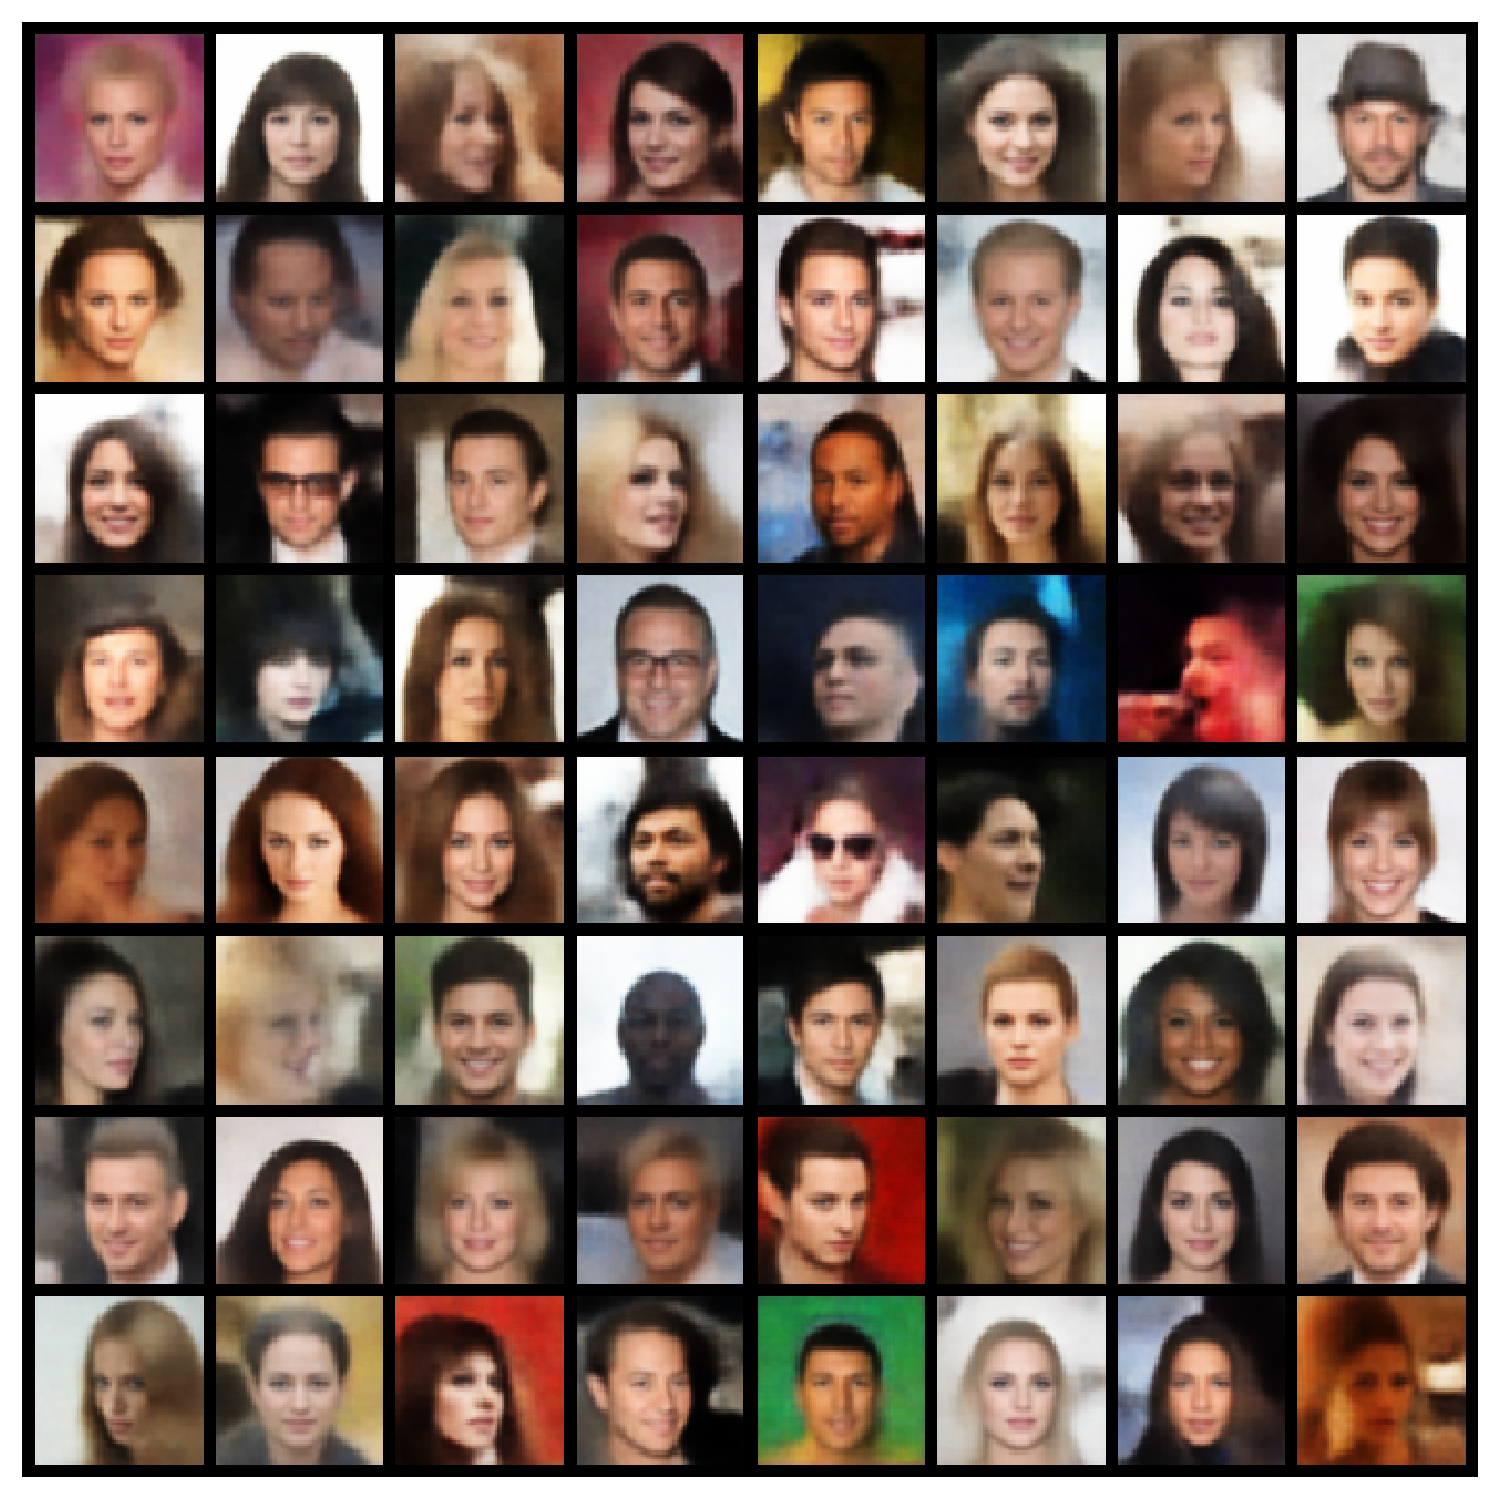
\includegraphics[width=.49\textwidth]{gfx/evaluation/celeba/fake-regular}
  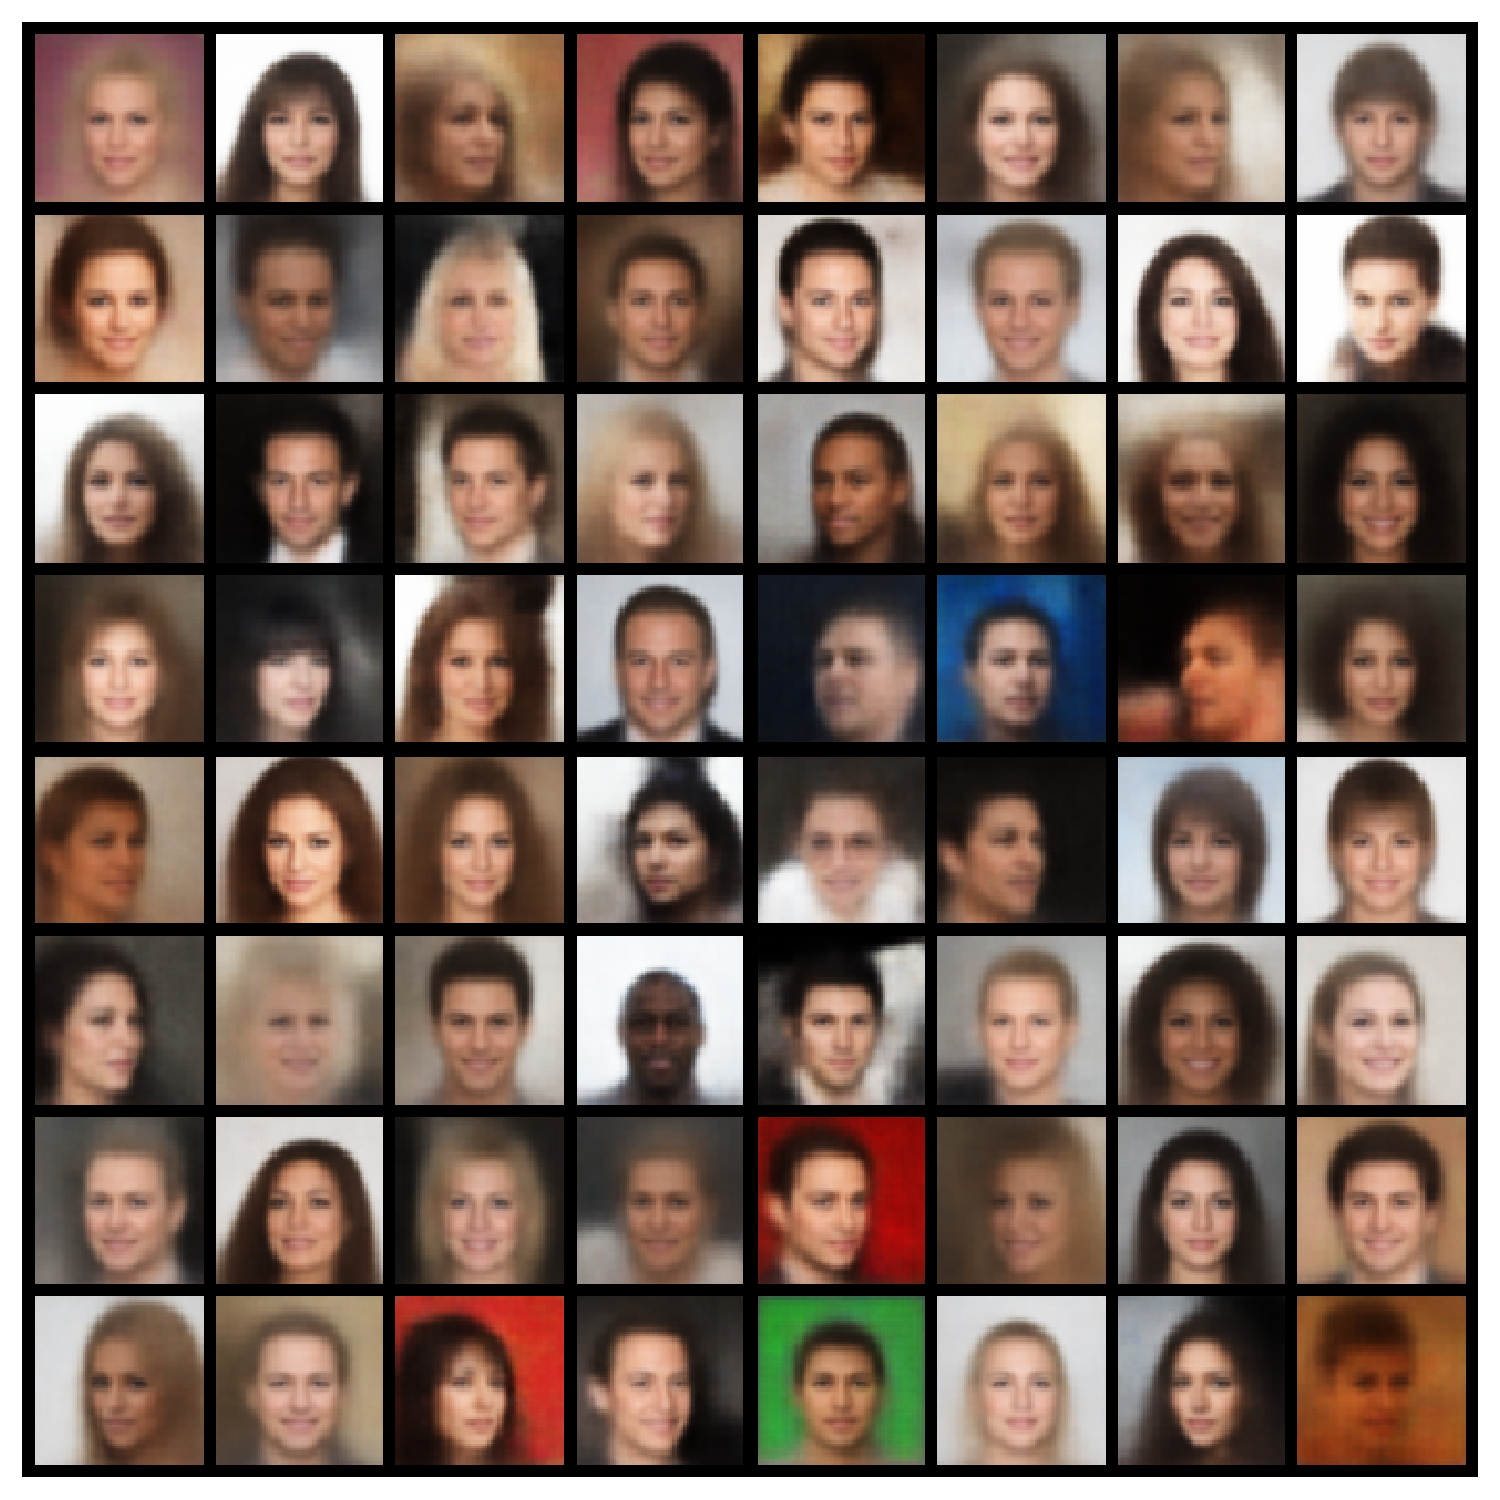
\includegraphics[width=.49\textwidth]{gfx/evaluation/celeba/fake-beta}
  \caption{CelebA - Originalbilder oben, Rekonstruktionen mit verschiedenen Werten für $\beta$ unten. $\beta_{norm}$ (links), $150 \cdot \beta_{norm}$ (rechts)}
  \label{fig:celeba_recon}
\end{figure}

In Abb. \ref{fig:celeba_disentangled} sind Interpolationen von beiden Modellen jeweils in einer Dimension zu sehen. Im oberen Bild stellt das interpolierte Merkmal eine Rotation von rechts nach links dar, im unteren Bild die Farbe der Haut. Man sieht, dass das Modell mit $\beta = 1$ Schwierigkeiten hat, die Merkmale "Hautfarbe" und "Lächeln" zu trennen. Dies ist bei dem Modell mit $\beta = 150$ nicht der Fall. Ein höherer $\beta$ Wert führt also zu Entwirrung von Merkmalen in den Dimensionen des Latent-Space. Erklären lässt sich das folgendermaßen (vgl. \cite{Higgins2017}): Durch den hoch gewichteten KL-Term wird die vom Encoder gebildete Normalverteilung Richtung Erwartungswert 0 und Varianz 1 gezwungen. Dies führt dazu, dass die Trennung von Merkmalen nun mehr über Dimensionen erfolgen muss. Daher sehen wir, dass verschiedene Dimensionen unterschiedliche Merkmale kontrollieren. Diese Repräsentation wird auch "Disentangled-Feature-Representation" genannt \cite{Higgins2017}. In Abb. \ref{fig:celeba_disentanglement_examples} sind weitere unabhängige Merkmale visualisiert.

\begin{figure}[hbt]
\centering
  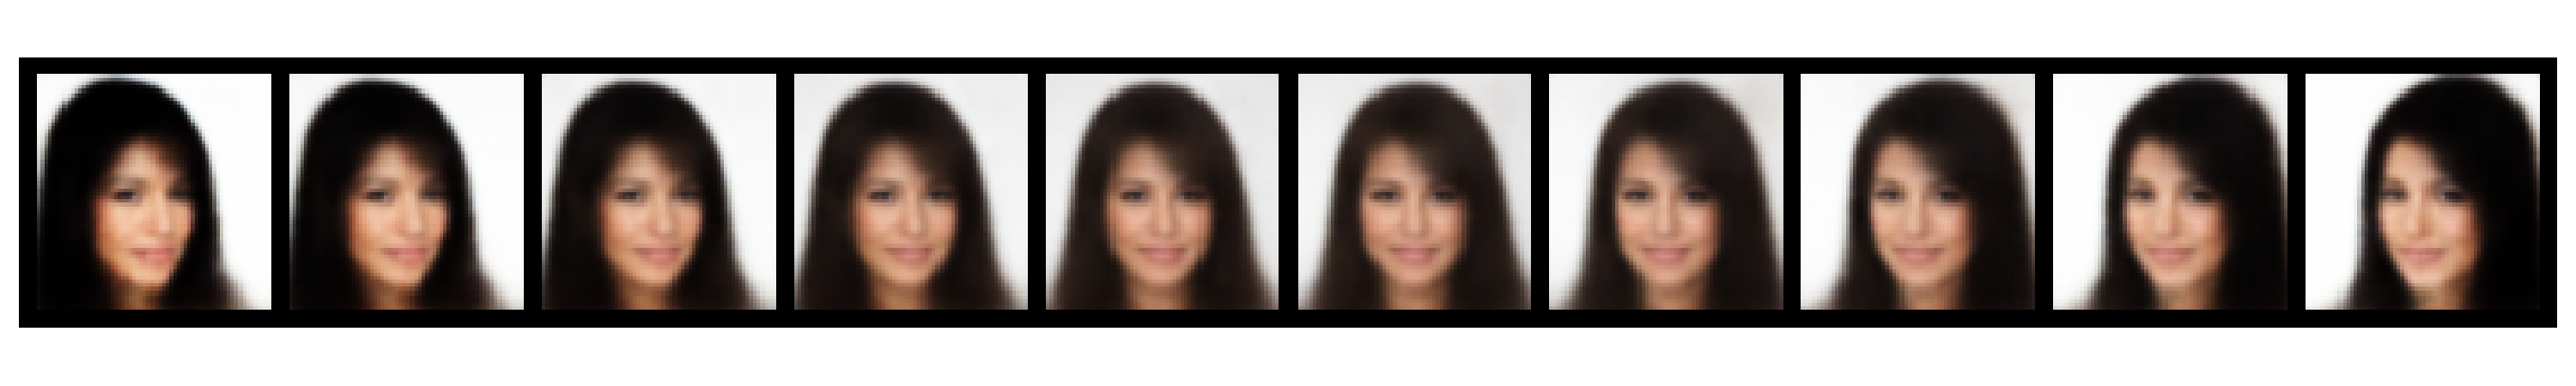
\includegraphics[width=.9\textwidth]{gfx/evaluation/celeba/CelebA-Rotation_1}
  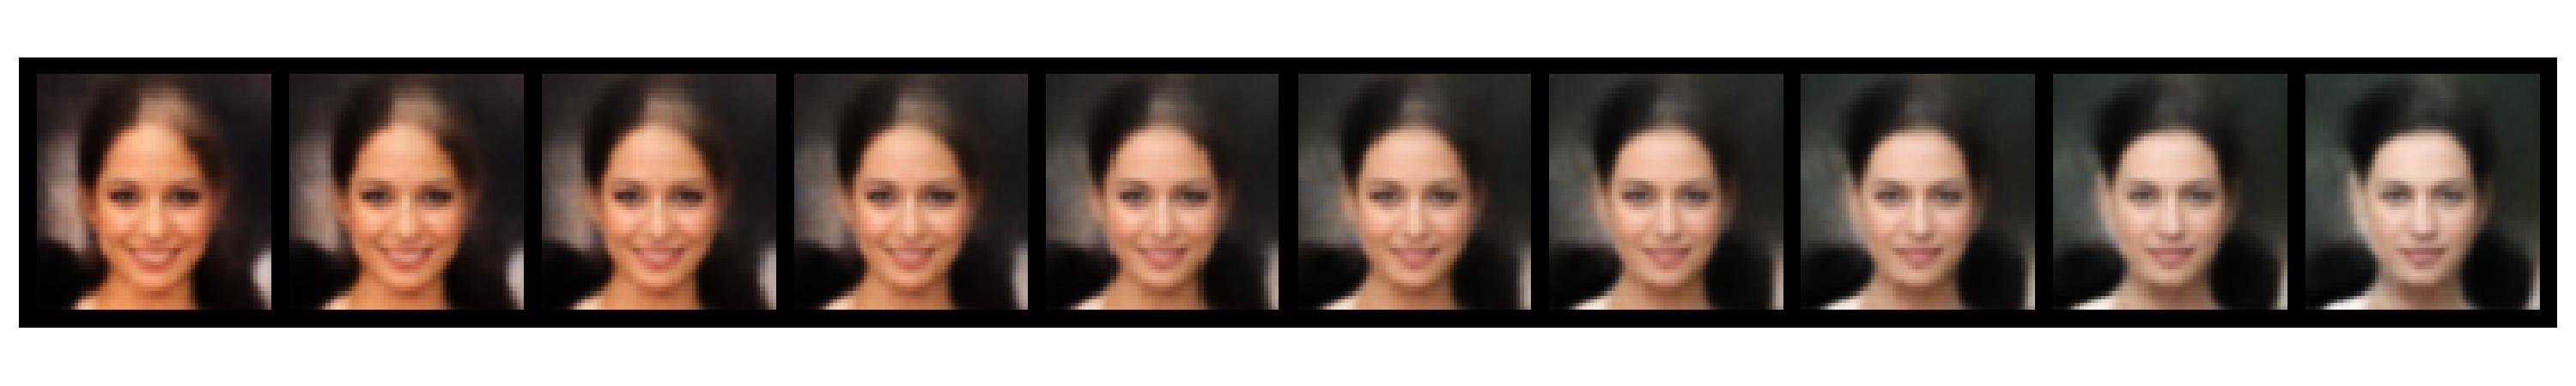
\includegraphics[width=.9\textwidth]{gfx/evaluation/celeba/regular-face-color}
  \caption{Sweep durch eine Dimension im Latent-Space für ein gegebenes Originalbeispiel (Die anderen Dimensionen sind fest). Oben zu sehen der VAE mit $\beta_{norm}$ für $\beta = 150$, unten $\beta_{norm}$ mit $\beta = 1$. Der höhere $\beta$ Wert erzielt eine bessere entkopplung der Merkmale. Unten zu sehen ist, dass das Merkmal "Hautfarbe" und "Lächeln" gekoppelt sind.}
  \label{fig:celeba_disentangled}
\end{figure}

\begin{figure}[H]
  \centering
  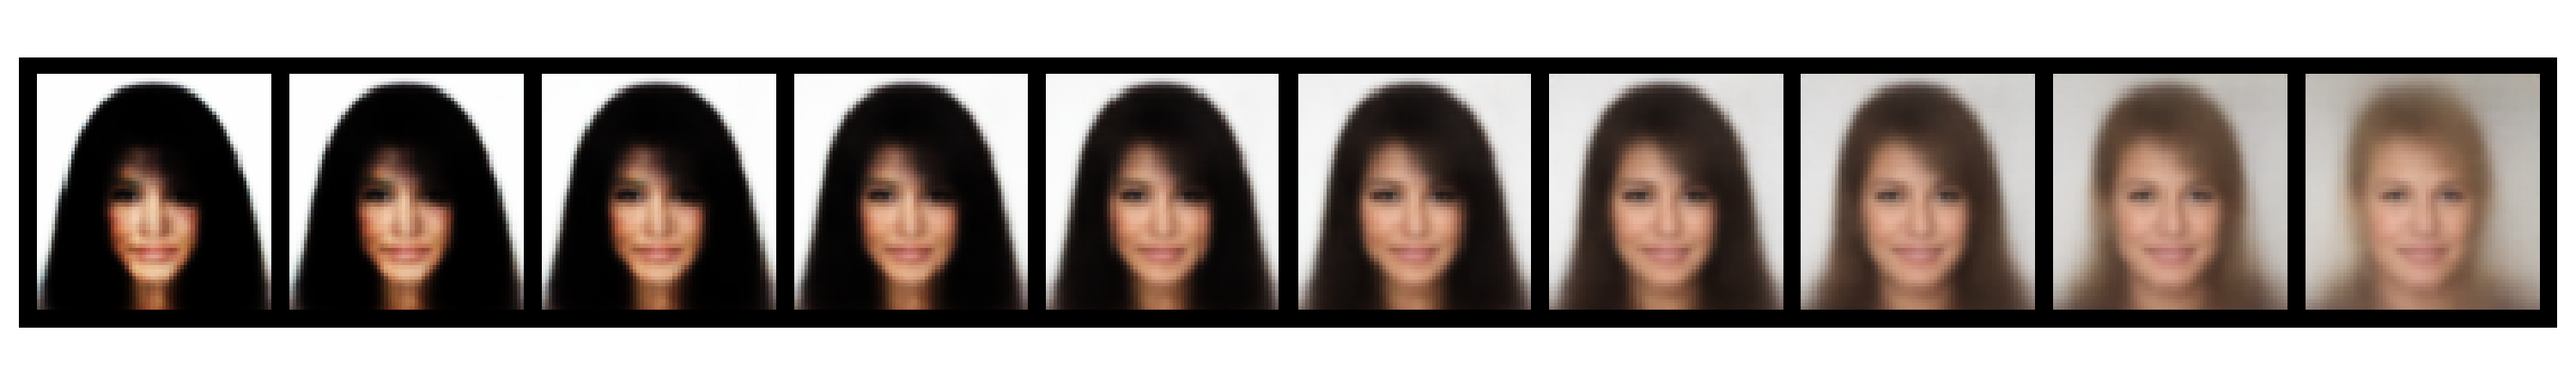
\includegraphics[width=.9\textwidth]{gfx/evaluation/celeba/CelebA-hair-color_1}
  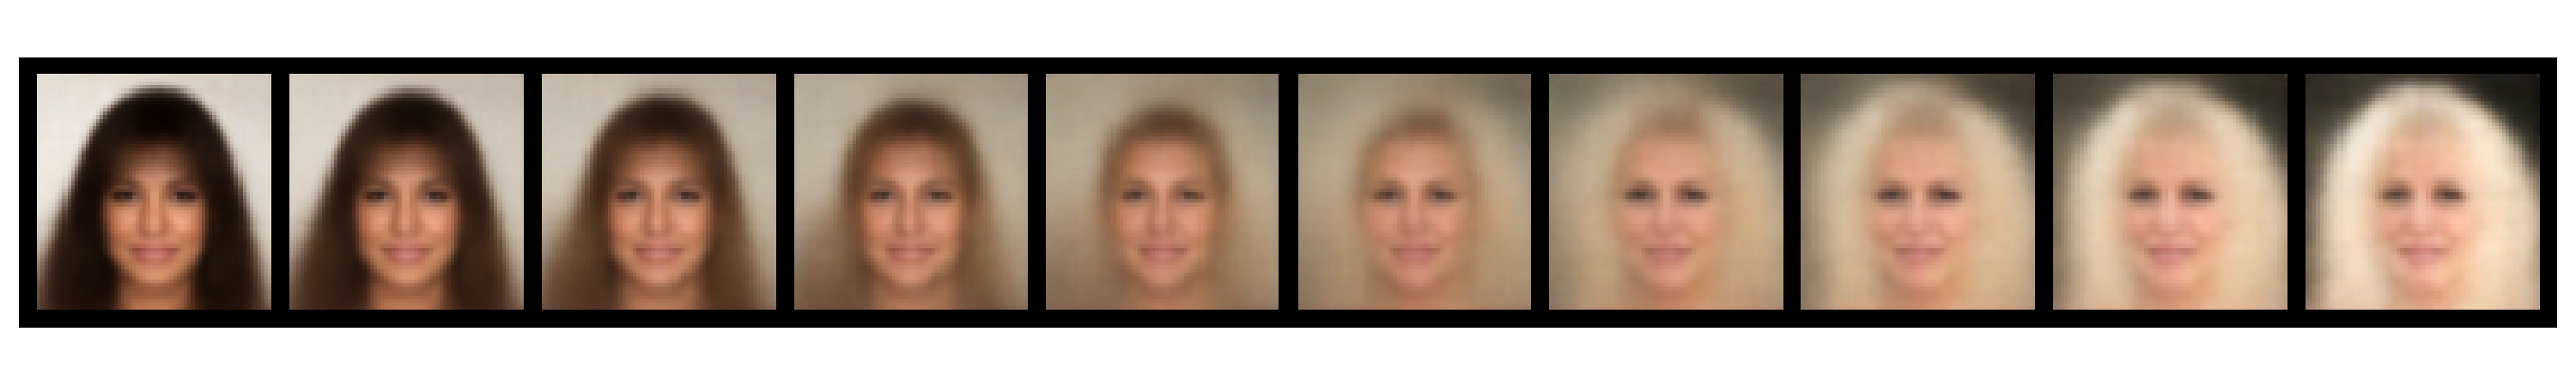
\includegraphics[width=.9\textwidth]{gfx/evaluation/celeba/CelebA-hair-color_3}
  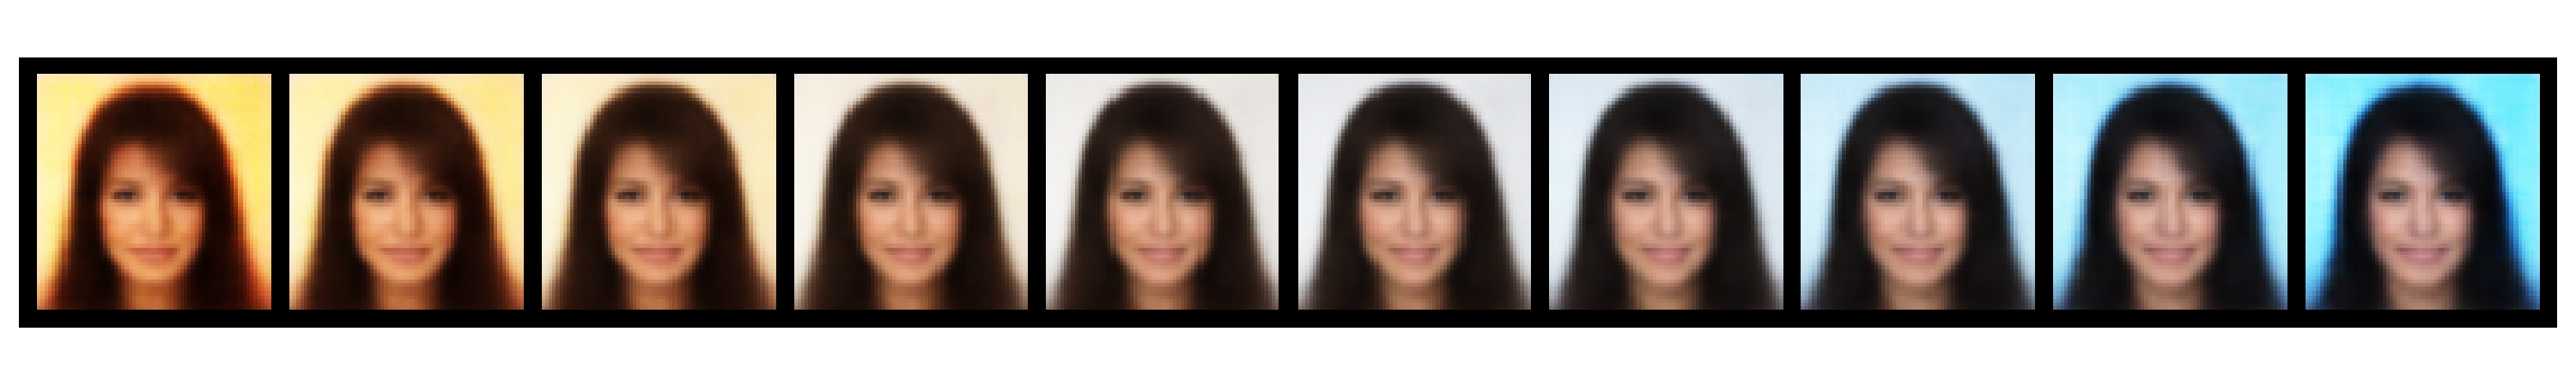
\includegraphics[width=.9\textwidth]{gfx/evaluation/celeba/CelebA-bg-color_1}
  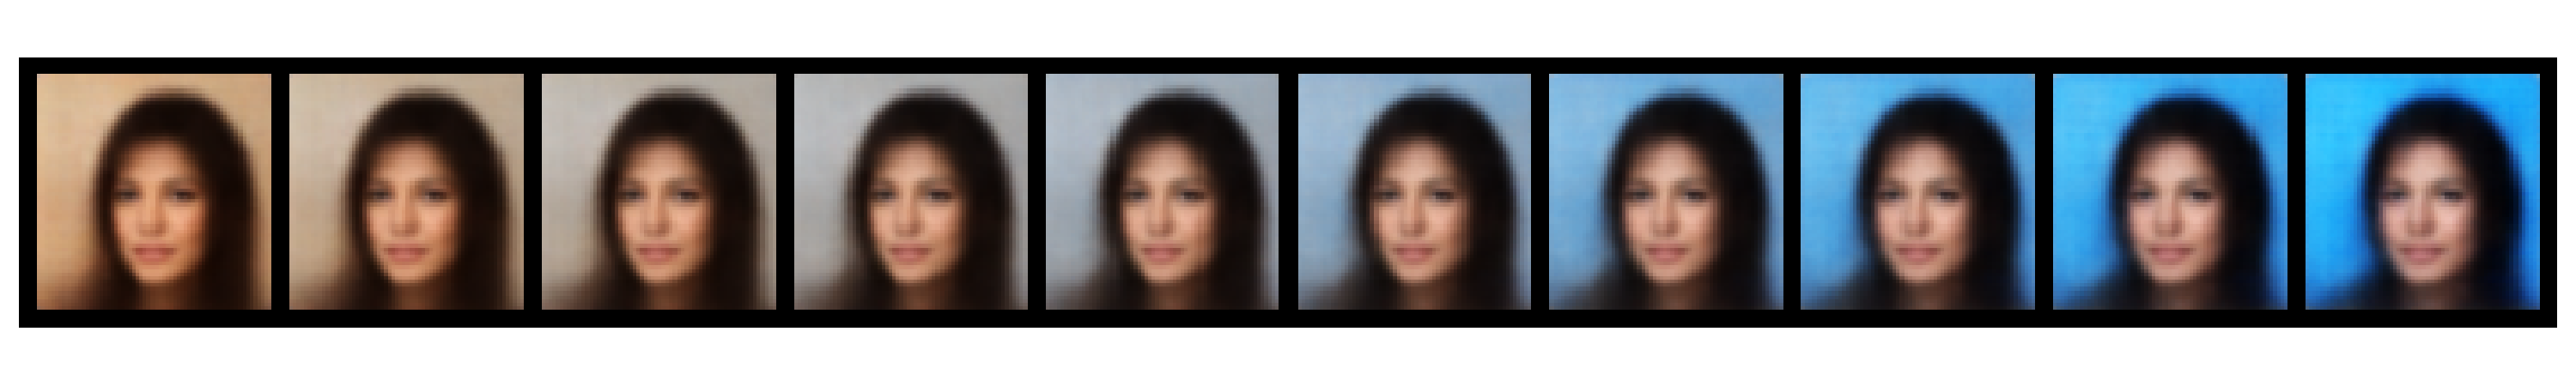
\includegraphics[width=.9\textwidth]{gfx/evaluation/celeba/CelebA-bg-color_3}
  \caption{Weitere entkoppelte Dimensionen des \textit{Disentangled}-VAE. Oben: Das Merkmal "Haarfarbe". Unten: Die Hintergrundfarbe.}
  \label{fig:celeba_disentanglement_examples}
\end{figure}



\section{Limitationen von VAE}
In den durchgeführten Experimenten ist aufgefallen, dass die Rekonstruktionen, welche der VAE erzeugt, unscharf sind. Dies betrifft vor allem den Hintergrund bei den Daten des CelebA Datensatzes. Für Datensätze, welche keine organischen Merkmale wie Gesichtszüge besitzen, ist dieser Effekt noch stärker ausgeprägt. Dies ist z.B. beim CIFAR-10 Datensatz der Fall (siehe Abb. \ref{fig:cifar10-bad-recon}).

\begin{figure}[H]
  \centering
  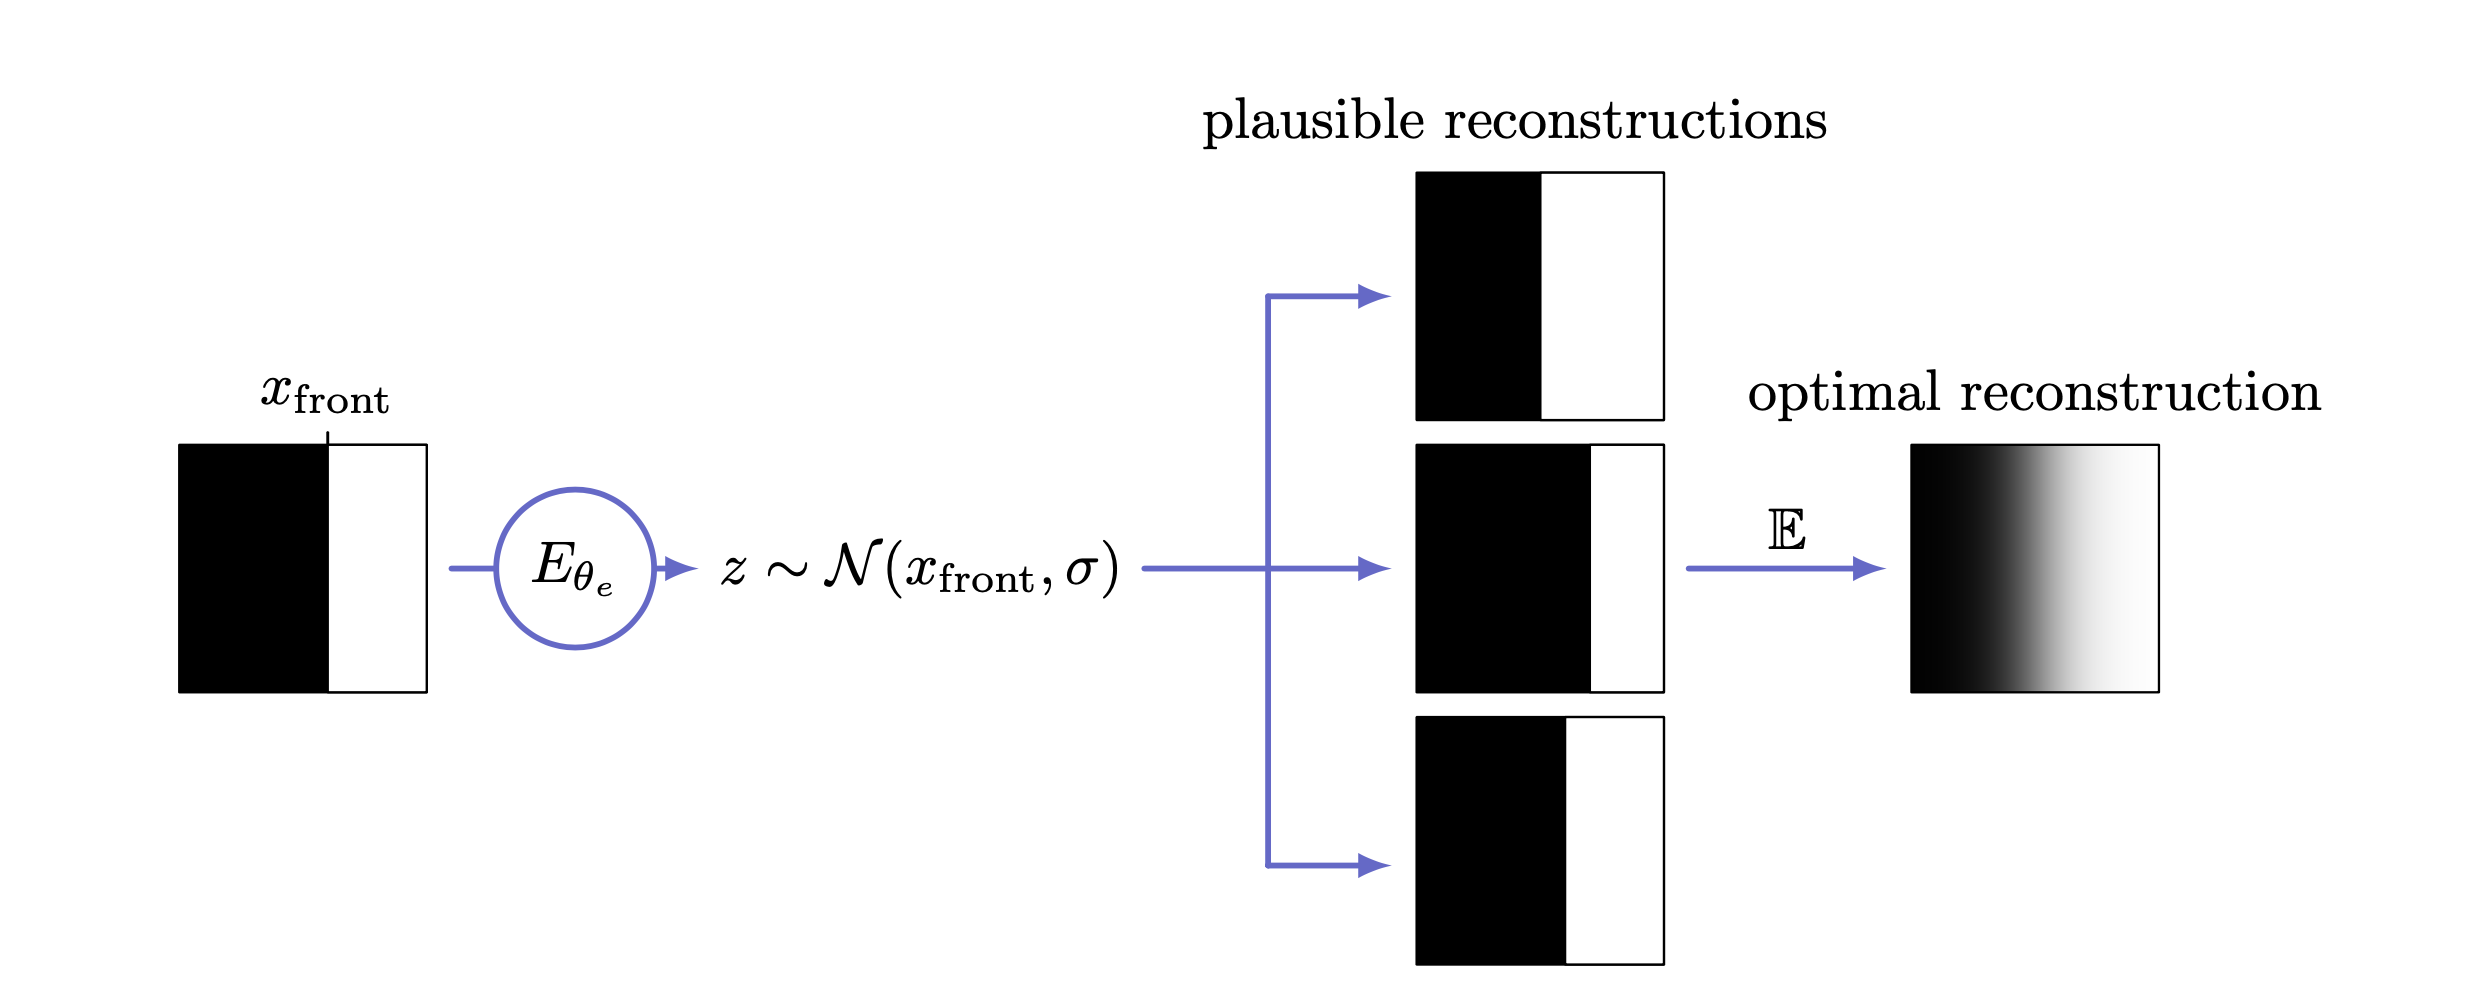
\includegraphics[width=.9\textwidth]{gfx/evaluation/recon_blur}
  \caption{Grund für die unscharfen Rekonstruktionen des VAEs ist die Modellierung der Ausgabe über eine Verteilung im Latent-Space. Damit sind mehrere Rekonstruktionen plausibel und ergeben eine unscharfe optimale Rekonstruktion.}
  \label{fig:blur_explained}
\end{figure}

Eine Erklärung für dieses Phänomen bei VAEs liefern \cite{Plumerault2020} (siehe Abb. \ref{fig:blur_explained}). Betrachtet wird eine Kante im Eingabebild $i$ und der Latent-Vektor $z$, welcher die Position $x_{front}$ der Kante beschreibt. Wenn nun 
\[
Q_\phi(z \vert i) = \cN(x_{front}, \sigma)
\]
, dann ist die Verteilung der plausiblen Rekonstruktionen gegeben durch
\[
P_\theta(x_{front} \vert z) = \cN(z, \sigma)
\]. Die optimale Rekonstruktion des betrachteten Pixels ist durch den Erwartungswert über diese Verteilung gegeben, was einem weichen Übergang entspricht.

\begin{figure}[hbt]
  \centering
  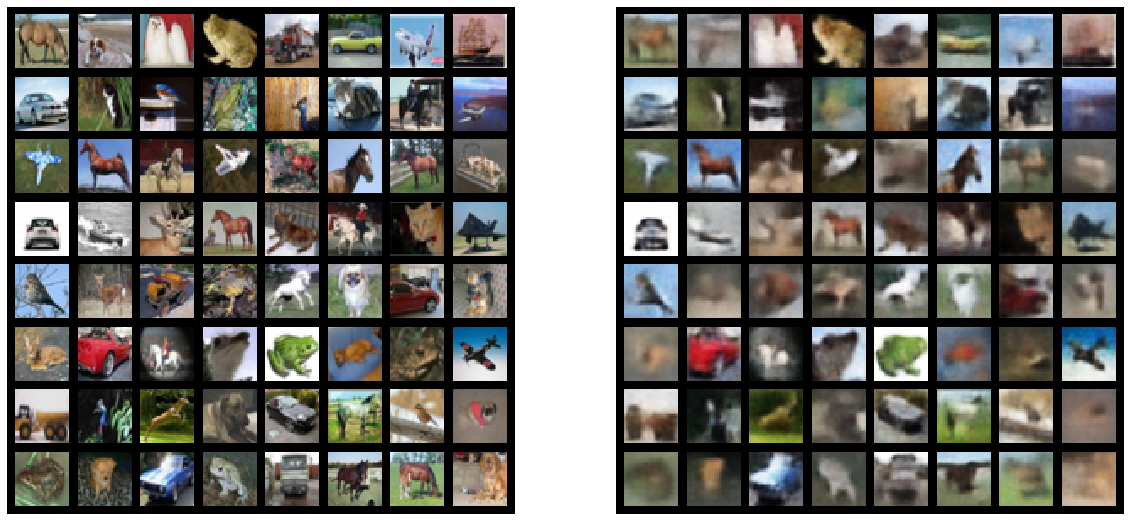
\includegraphics[width=\textwidth]{gfx/evaluation/cifar-10}
  \caption{Die Rekonstruktionen auf dem Datensatz CIFAR-10 sind besonders stark von der unschärfe des VAEs betroffen. In einigen Fällen ist die Klasse nicht mehr ableitbar.}
  \label{fig:cifar10-bad-recon}
\end{figure}


